\documentclass{beamer}
\usepackage{xcolor}
\usepackage{natbib} % package to organize literature
\usepackage{booktabs}
\usepackage{graphicx} % to include graphics, gifs
\usepackage{lmodern} % to fix font size error, might be problematic with math symbols
\usepackage{tikz}
\usepackage{enumerate}
\usepackage{arydshln} % dashed lines
\usepackage{appendixnumberbeamer} % separate appendix numbering
\usepackage{fontawesome} % awesome icons
\usepackage[absolute,overlay]{textpos} % textbox in front of content
\usepackage{tabularx}

% Custom beamer settings
%\definecolor{beamer@sbred}{rgb}{0.65,0.15,0.18}
\definecolor{beamer@sbred}{rgb}{0.22,0.22,0.66}
\setbeamercolor{structure}{fg=beamer@sbred}
\setbeamertemplate{itemize items}[default]
\setbeamertemplate{enumerate items}[default]
\setbeamersize{text margin left=1em,text margin right=1em}
\setbeamercolor{frametitle}{fg=beamer@sbred}
\setbeamercolor{section in toc}{fg=beamer@sbred}
\setbeamercolor{subsection in toc}{fg=beamer@sbred!50}
\setbeamercolor*{block title example}{fg= white, bg= beamer@sbred!90}
\setbeamercolor*{block body example}{fg= black, bg= beamer@sbred!10}
\DeclareTextFontCommand{\emph}{\color{beamer@sbred}}

% link to table of contents
\makeatletter
\setbeamertemplate{footline}
{
	\leavevmode%
	\hbox{%
		\begin{beamercolorbox}[wd=.2\paperwidth,ht=2.25ex,dp=1ex,center]{}%
			\hyperlink{sec:main-content}{\emph{Content}} /  \hyperlink{sec:appendix-content}{\emph{Appendix}}
		\end{beamercolorbox}%
		\begin{beamercolorbox}[wd=.8\paperwidth,ht=2.25ex,dp=1ex,right]{date in head/foot}%
			%   \usebeamerfont{date in head/foot}\insertshortdate{}\hspace*{2em}
			\insertframenumber{} \hspace*{2ex}  / \hspace*{2ex} \inserttotalframenumber
			\hspace*{2ex} 
	\end{beamercolorbox}}%
	\vskip0pt%
}
\makeatother
\setbeamertemplate{navigation symbols}{}

\author{Patrick W. Kraft}
\title{Change My View\\
{\large Do Moral Appeals Facilitate Compromise?}}
\institute{MAPPS Meeting\\Marquette University}
\date{October 12\textsuperscript{th} 2018}
\titlegraphic{\includegraphics[width=3cm]{/data/Dropbox/Uni/Misc/Logos/UWM/UWM_preferred.png}}



\begin{document}


\section{Introduction}

\frame{\titlepage}

\begin{frame}{Introduction}
\begin{figure}
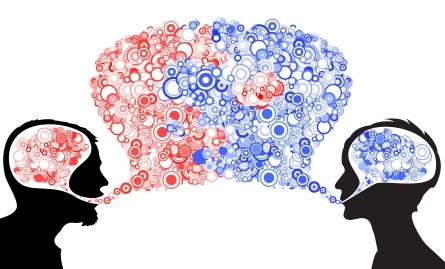
\includegraphics[scale=.9]{fig/the-conversation.jpeg}
\end{figure}
\end{frame}
% - My background: political psychology
% - I study how people describe and justify their political preferences
% - Ultimately, I am interested in exploring how citizens engage in political discussions and influence each other's opinions
% - Why does this matter?


\section{Theory}

\begin{frame}{How Can We Overcome Political Disagreements?}
\begin{figure}

\includegraphics[width=\textwidth]{fig/polarization_large.jpeg}
\end{figure}
\end{frame}
% - Politics in the US has become increasingly polarized
% - There are increasing levels of affective polarization and negative partisanship
% - Research: tribal politics can be overcome by fostering social interaction
% - Conversations with people who holds different views increases mutual understanding and trust
% - But can conversations in heterogeneous networks decrease the growing ideological divide?
% - Research in moral psychology suggests that it might not be that easy!
% - Politics is becoming increasingly moralized

\begin{frame}{Political Disagreements and Moral Considerations}
\begin{itemize}
	\item<1-> \emph{Moral Conviction literature}:\\Liberals and conservatives are less likely to compromise if they hold moral convictions about politics.\\
	{\footnotesize\citep[e.g.,][]{skitka2014social,ryan2017no}}\\
	\vspace{1em}
	\item<2-> \emph{Moral Foundations literature}:\\Liberals and conservatives are more likely to compromise if they focus on the same moral foundations.\\
	{\footnotesize\citep[e.g.,][]{graham2009liberals,haidt2012righteous}}
\end{itemize}
\end{frame}
% - Moral conviction literature says that we have to get morality out of politics to find agreement
% - Moral foundations literature says that we can overcome disagreements as long as we focus on the same moral foundations
% - Morality is always bad and counterproductive vs. morality can actually bring us together under the right circumstances.


\section{Online Discussions and Description of Dataset}

\begin{frame}{Analyzing Online Discussions}
\begin{figure}
	\only<1>{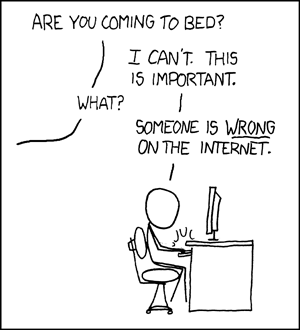
\includegraphics[height=.6\textheight]{fig/duty_calls.png}}
	\only<2>{
\includegraphics[width=\textwidth]{fig/reddit-01.png}}
	%\only<3>{
\includegraphics[width=\textwidth]{fig/reddit_many.png}}
\end{figure}
\end{frame}
% - Online discussions as a perfect environment were people encounter very different viewpoints.
% - Wikipedia: Reddit is a social news aggregation, web content rating, and discussion website. Registered members submit content to the site such as links, text posts, and images, which are then voted up or down by other members. Posts are organized by subject into user-created boards called "subreddits", which cover a variety of topics including news, science, movies, video games, music, books, fitness, food, and image-sharing. Submissions with more up-votes appear towards the top of their subreddit and, if they receive enough votes, ultimately on the site's front page.

\subsection{The Subreddit \texttt{/r/ChangeMyView}}
\begin{frame}{The Subreddit \texttt{/r/ChangeMyView}}
\begin{figure}
	\only<1>{
\includegraphics[width=\textwidth]{fig/reddit-02.png}}
	\only<2>{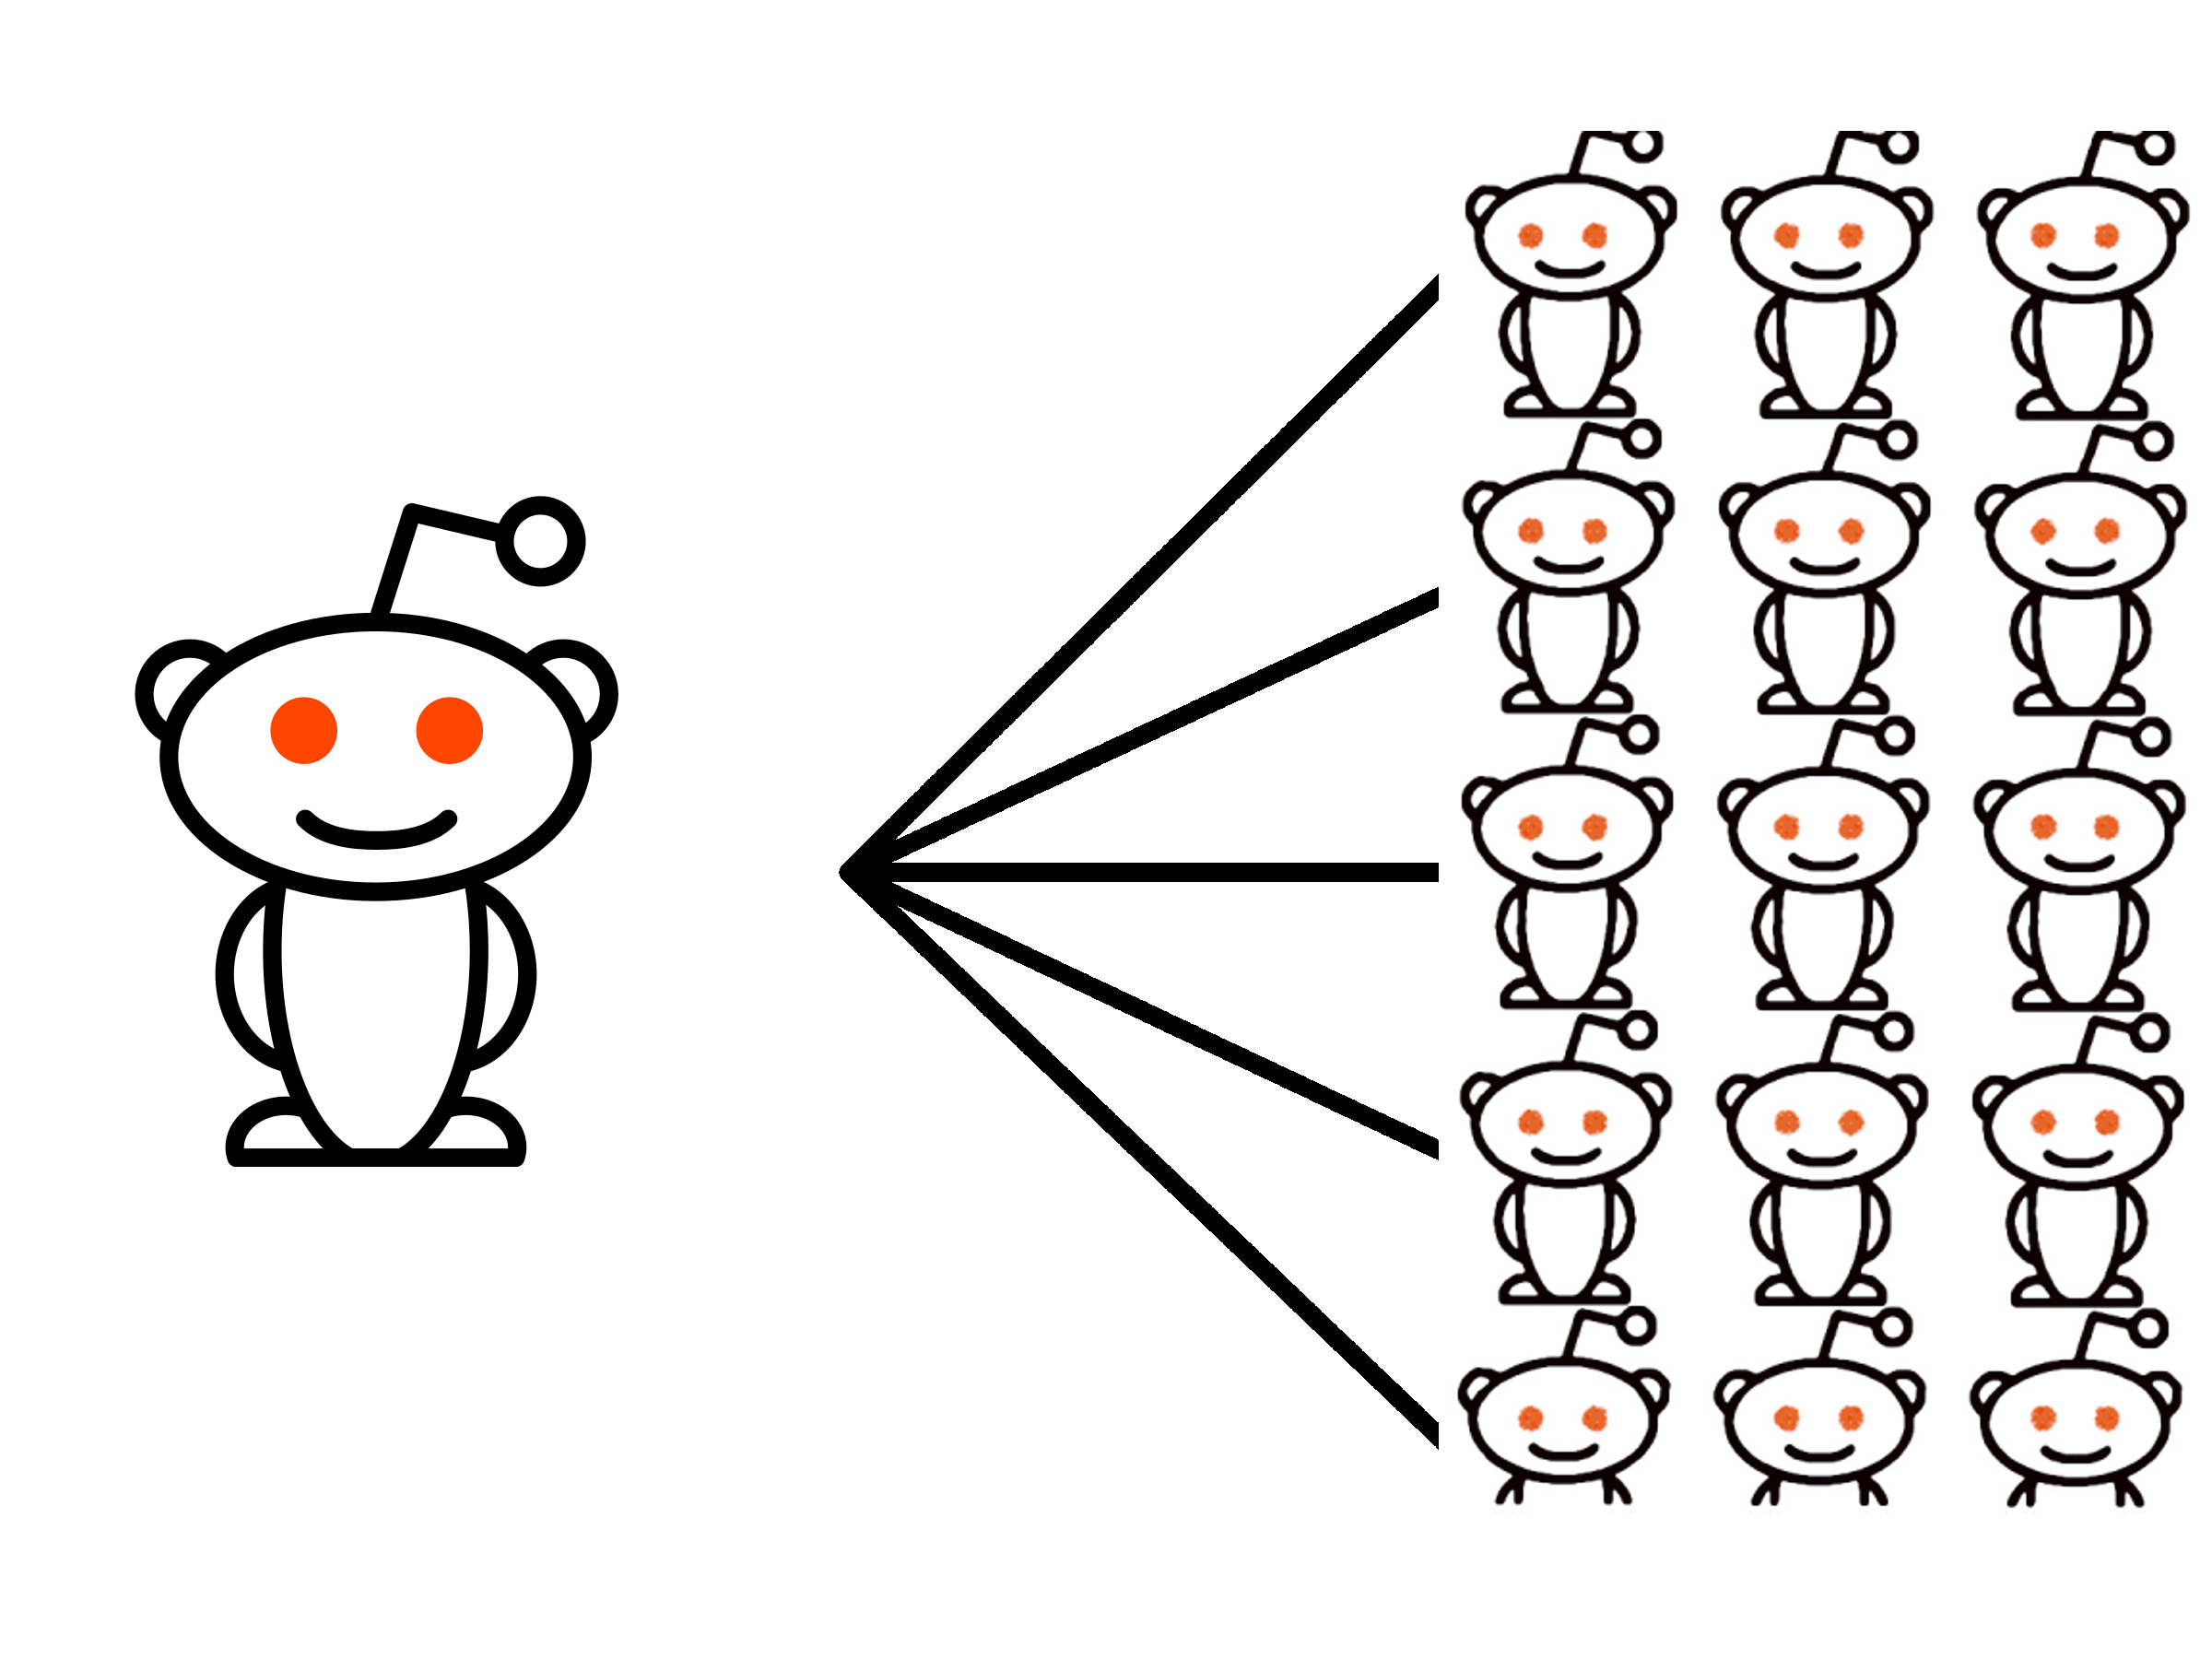
\includegraphics[width=\textwidth]{fig/reddit-03.png}}
	\only<3>{
\includegraphics[width=\textwidth]{fig/reddit-04.png}}
	\only<4>{
\includegraphics[width=\textwidth]{fig/reddit-05.png}}
	\only<5>{
\includegraphics[width=.95\textwidth]{fig/reddit_screenshot.png}}
\end{figure}
\end{frame}
% - Specifically, I am going to focus on a subreddit called ChangeMyView
% - In this subreddit, users can post their opinion about any issue (including a detailed justification) and other users are invited to challenge the original poster's view.
% - Most importantly, the OP then engages in discussions with the challengers and explicitly identifies posts that changed his or her mind by awarding a "Delta"
% - Here is a screenshot of the website that I took yesterday, we can see that the discussions cover a range of different topics, some of which are clearly political. Also note the rules on the side.

\subsection{Data Overview}
\begin{frame}{Data Overview}

Dataset of more than \emph{10,000 discussions} on \texttt{/r/ChangeMyView}: 
\begin{itemize}[<+->]
	\item Posted between January 2013 and May 2015
	\item Includes \emph{matched pairs} of successful and unsuccessful arguments
	\item Compiled by \citet{tan2016winning}, who studied \emph{linguistic features} (e.g., use of personal pronouns) and \emph{differences in style} (formatting etc.) that predict persuasiveness
	\vspace{1em}
	\item \emph{This analysis}: Exploring the role of \emph{moral appeals} in facilitating or inhibiting compromise
\end{itemize}
\end{frame}


\section{Empirical Results}

\subsection{Opening Statements and Persuadability}
\begin{frame}{Extracting Topics from Text -- Latent Dirichlet Allocation}
\begin{figure}
	\only<2>{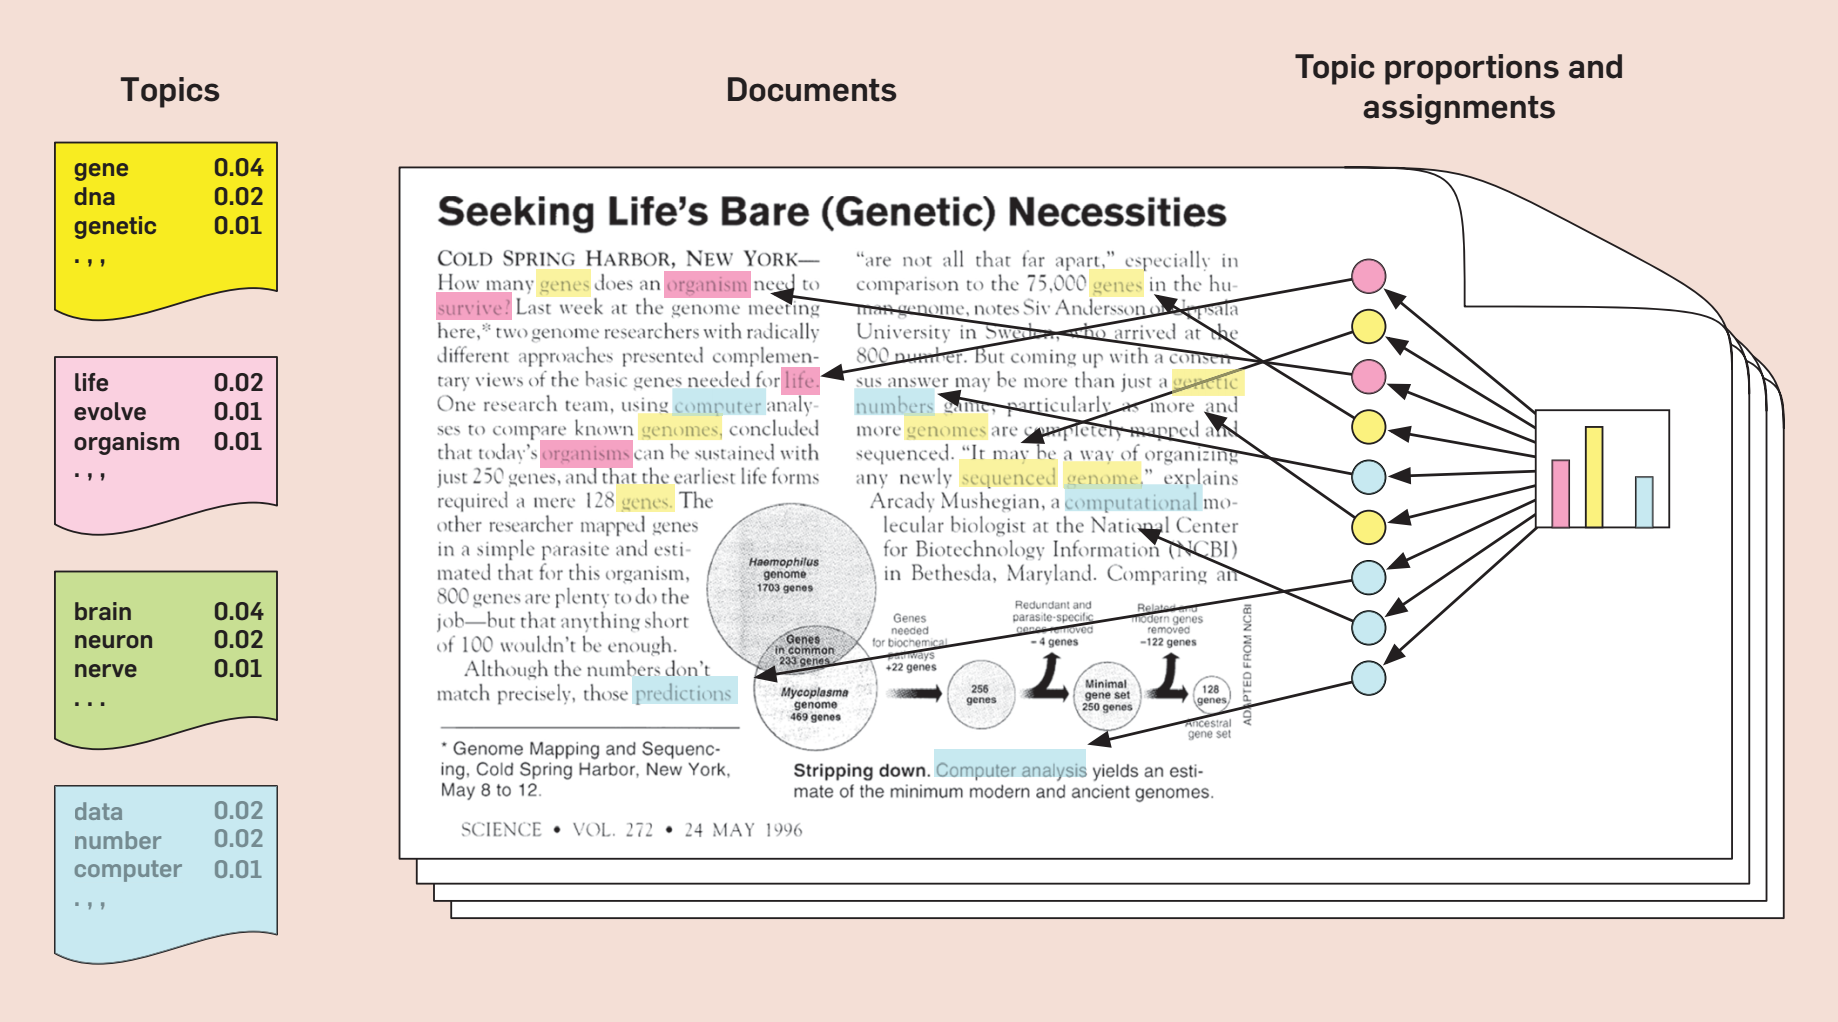
\includegraphics[width=\textwidth]{fig/blei2012probabilistic.png}}
\end{figure}
\only<2>{\tiny{\textit{Source:} \cite{blei2012probabilistic}}}
\end{frame}

\begin{frame}{Discussion Topics on \texttt{/r/ChangeMyView}}
\begin{figure}
\only<1>{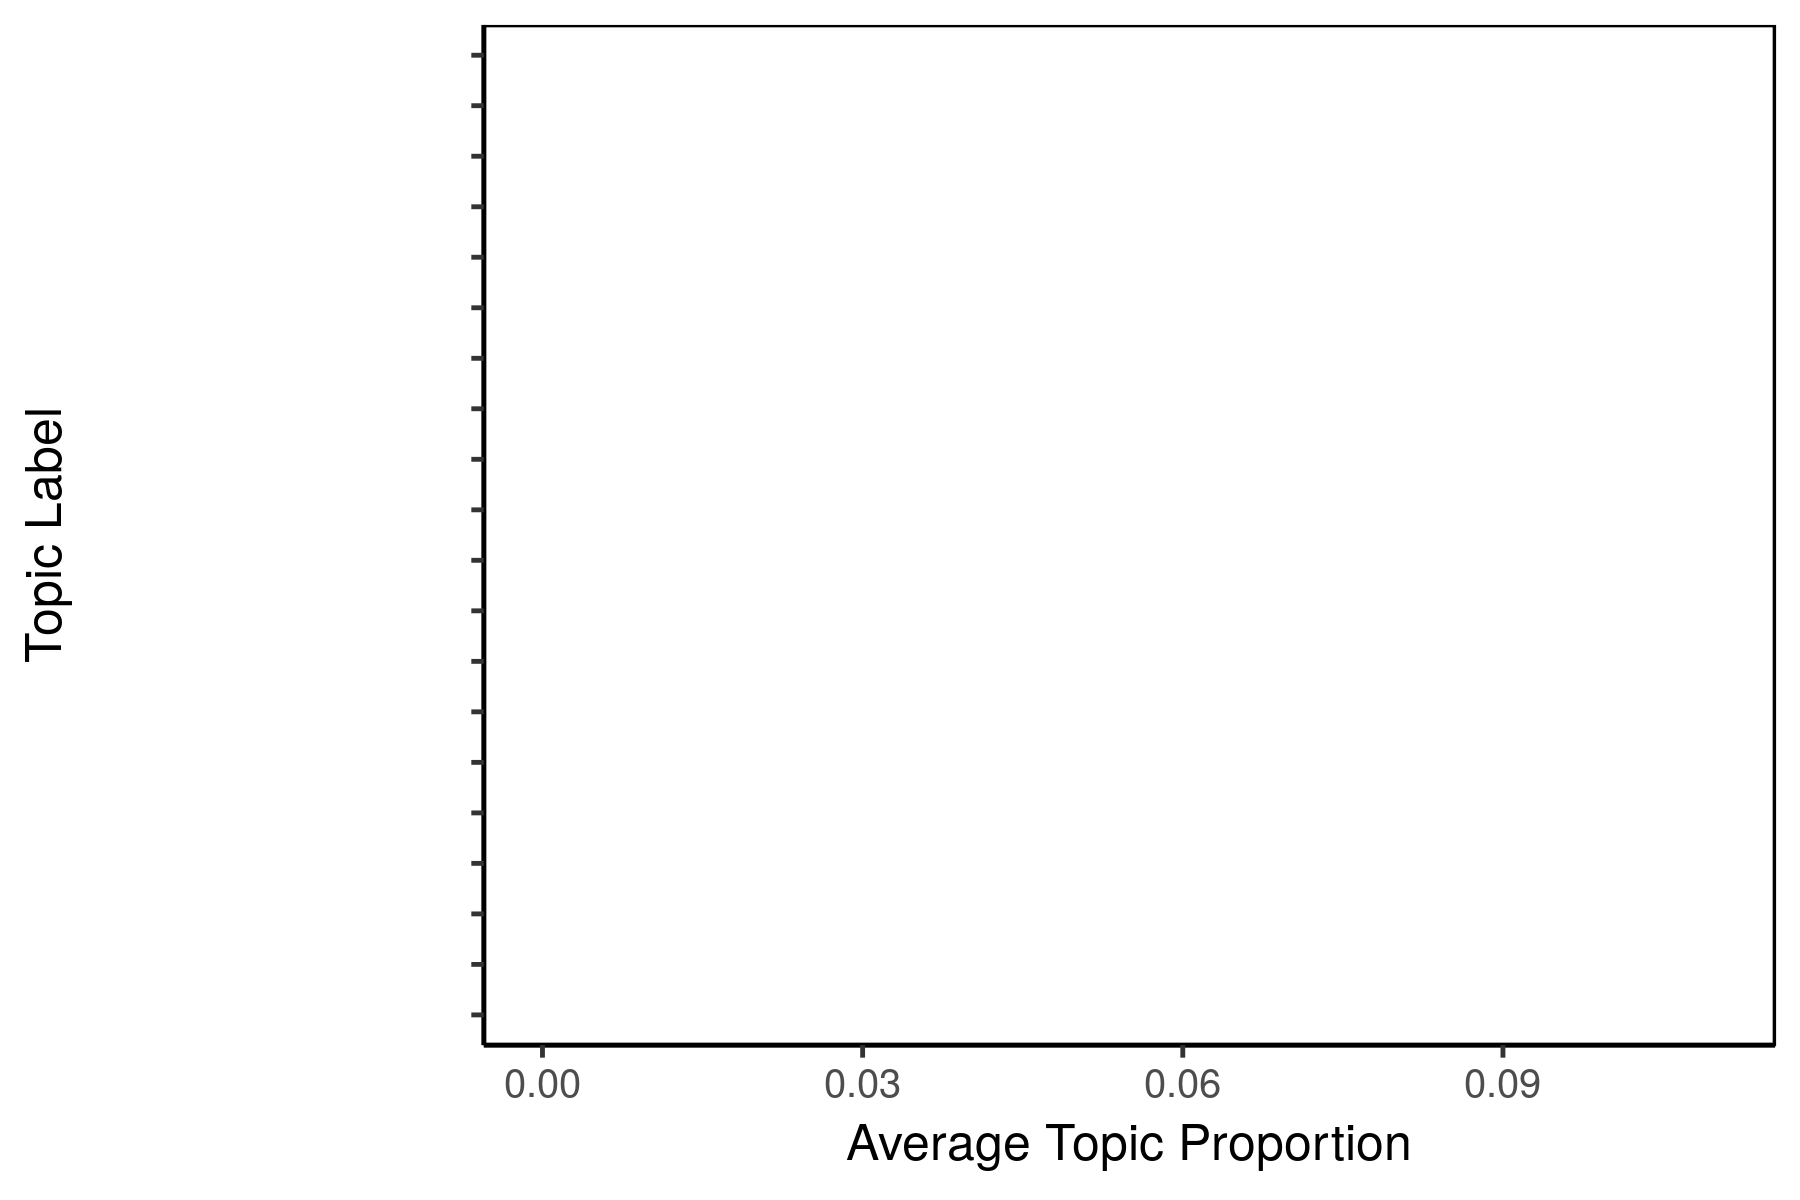
\includegraphics{../calc/fig/topics_00.png}}\only<2>{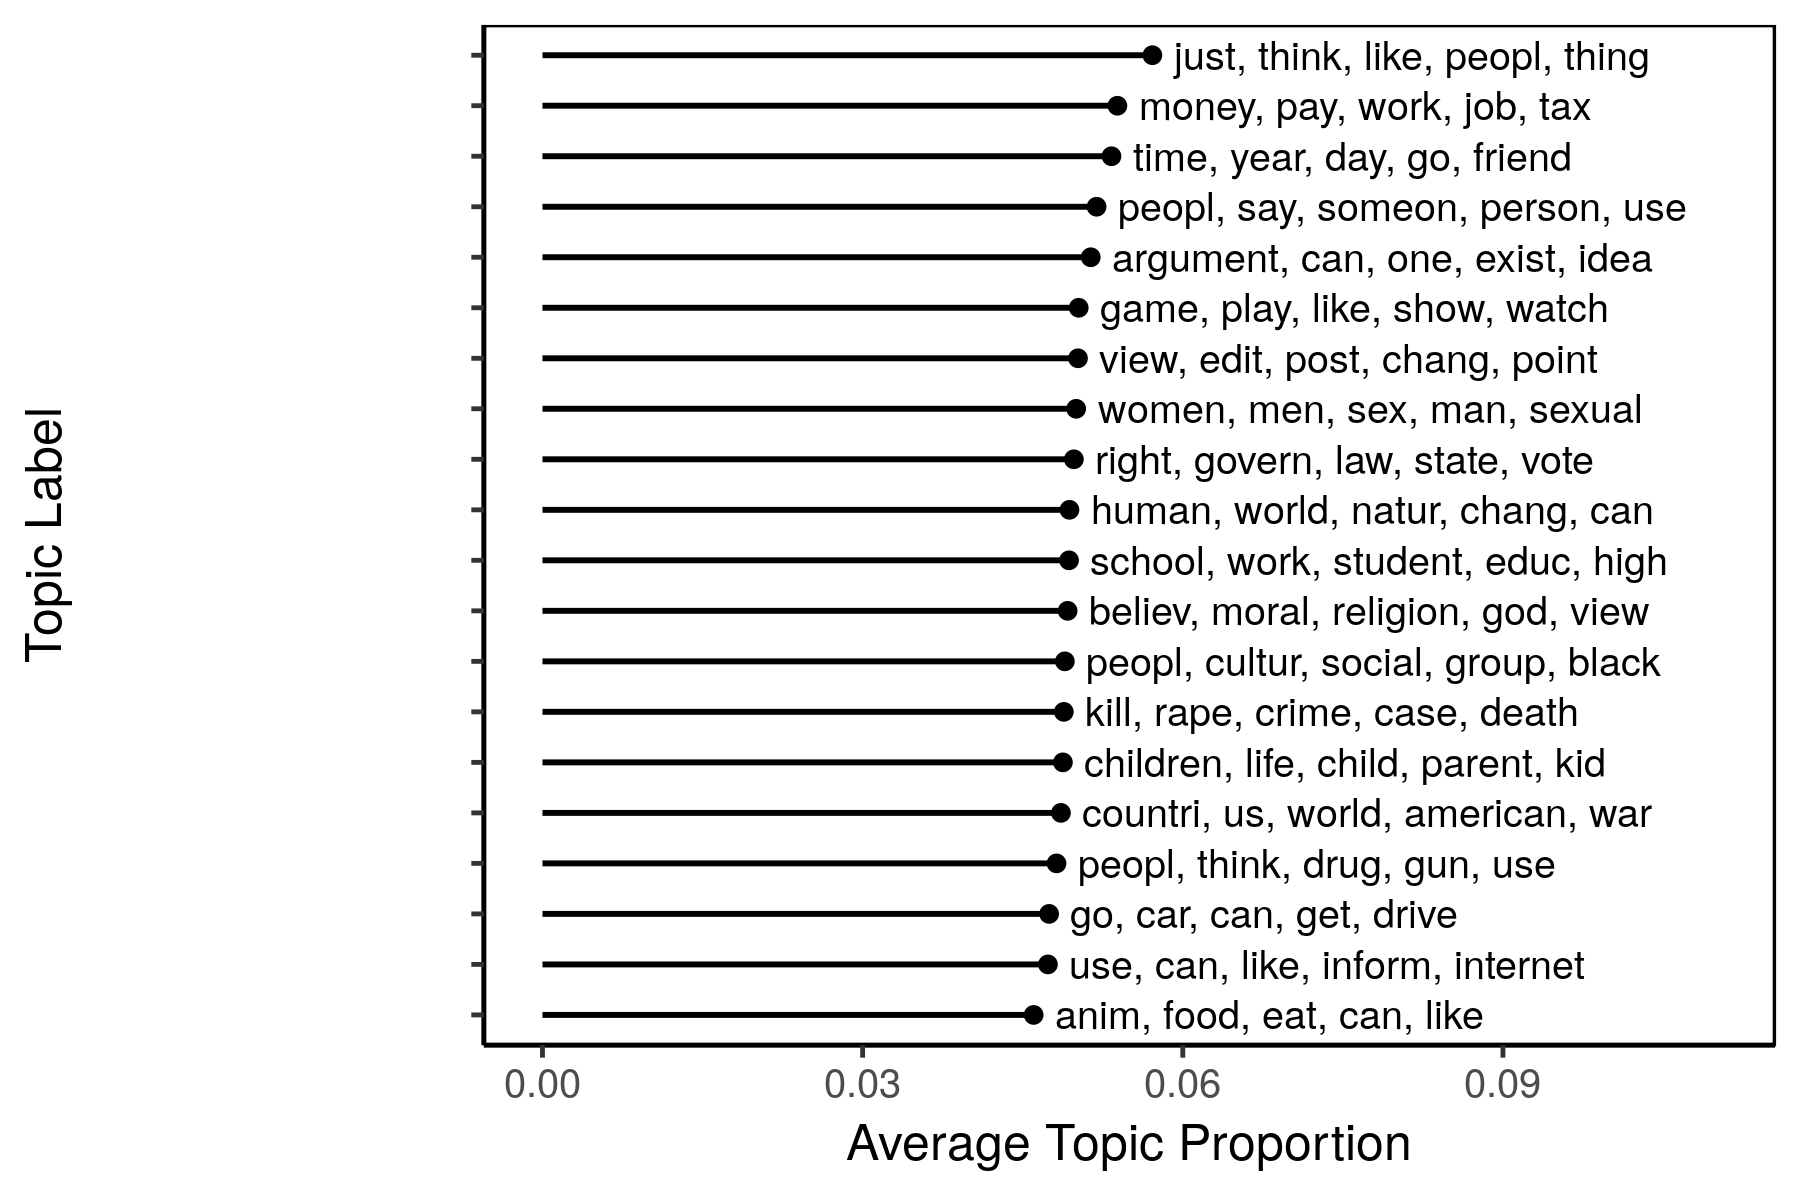
\includegraphics{../calc/fig/topics_01.png}}\only<3>{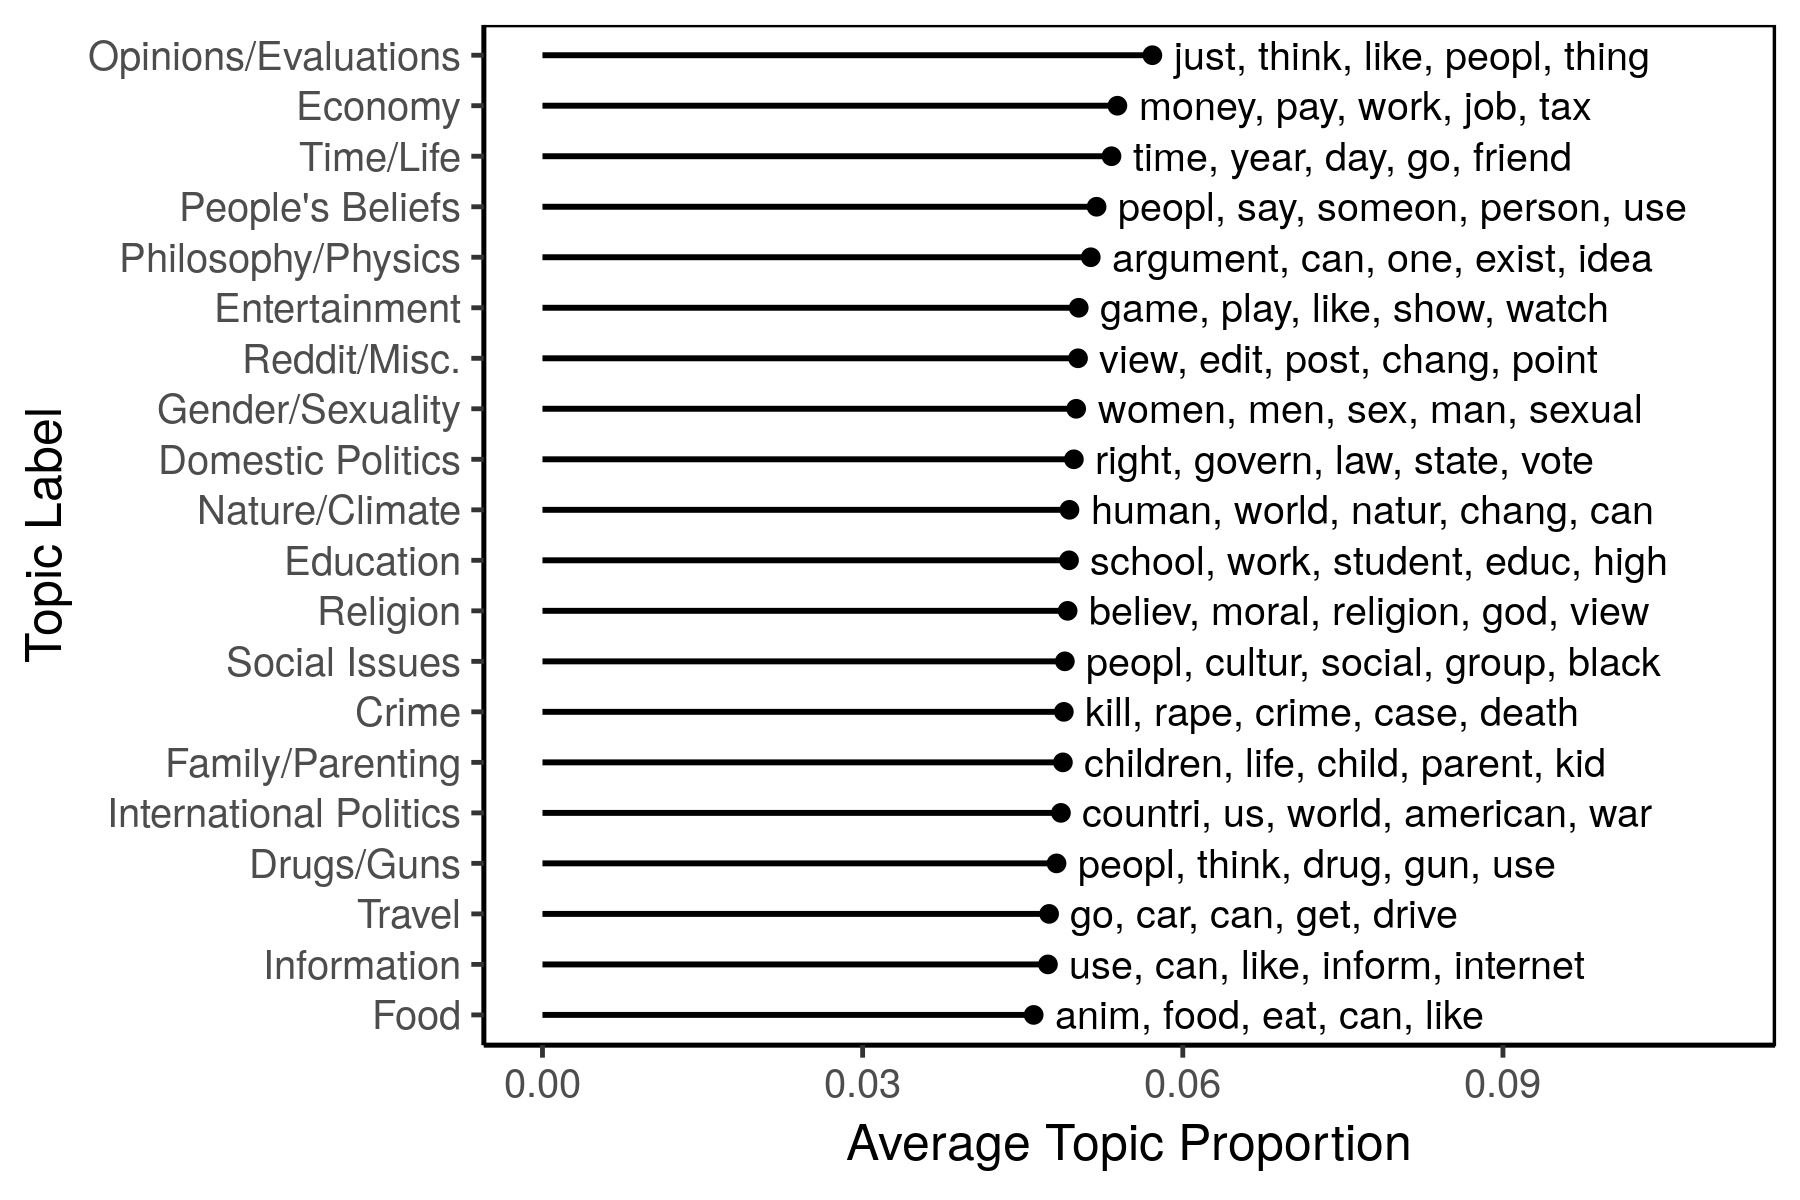
\includegraphics{../calc/fig/topics_02.png}}
\end{figure}
\end{frame}

\begin{frame}{Awarding $\Delta$s on \texttt{/r/ChangeMyView}}
\begin{figure}
\only<1>{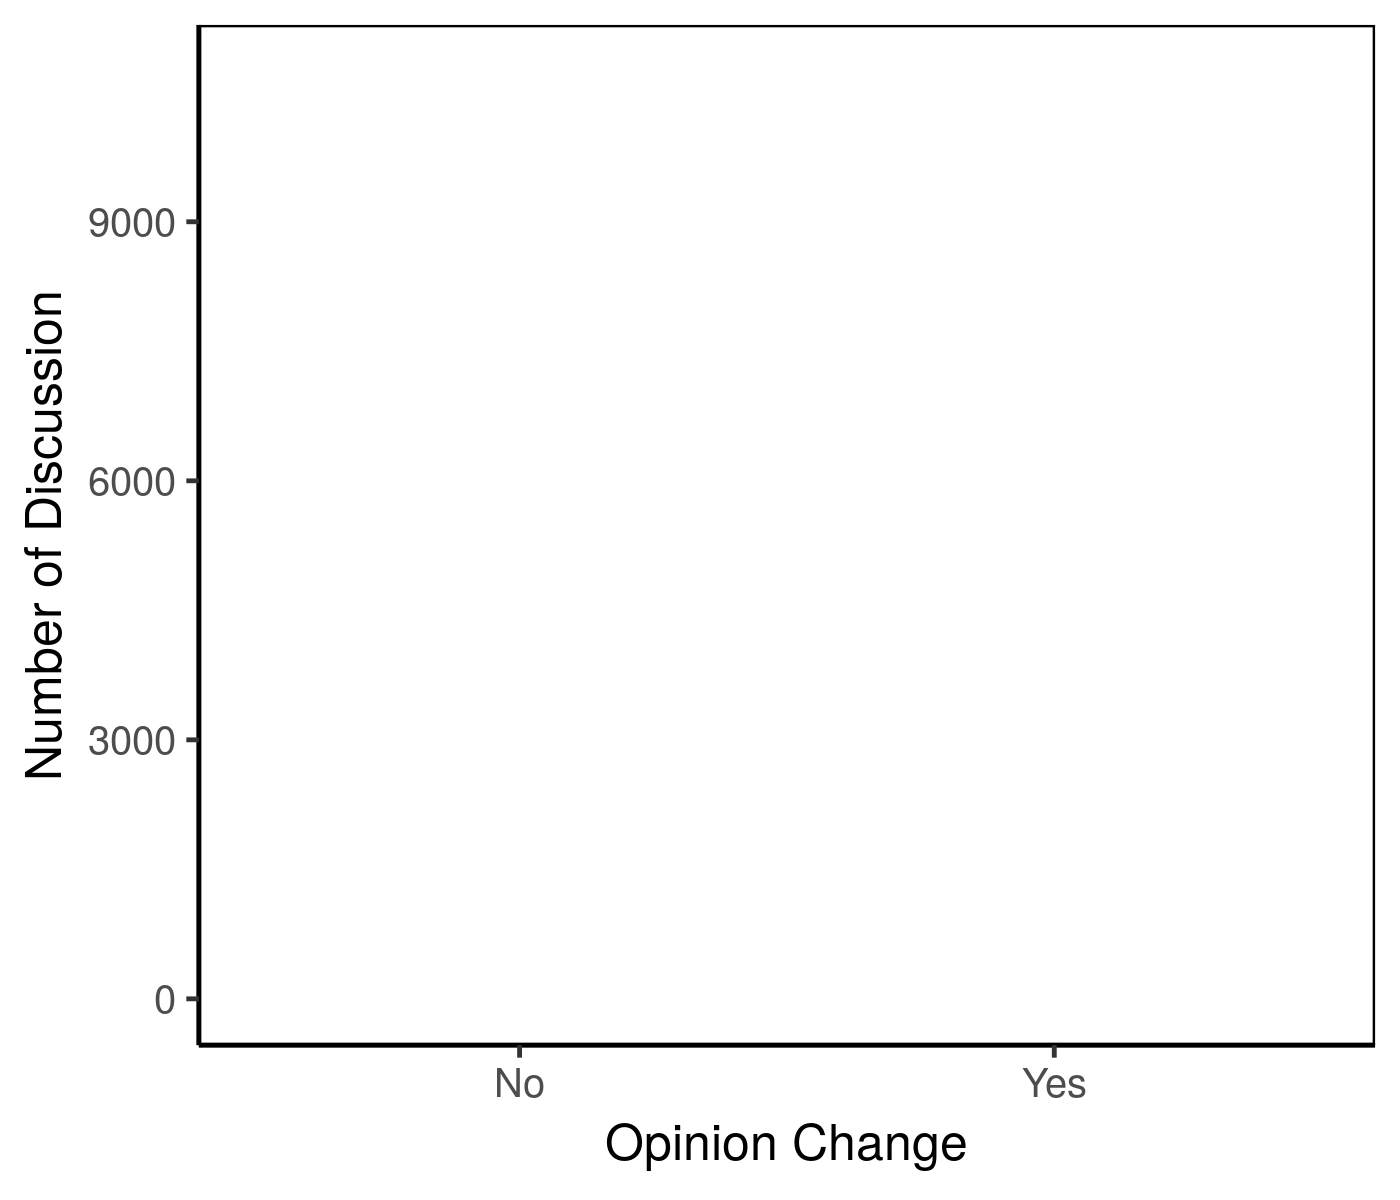
\includegraphics{../calc/fig/delta_empty.png}}\only<2>{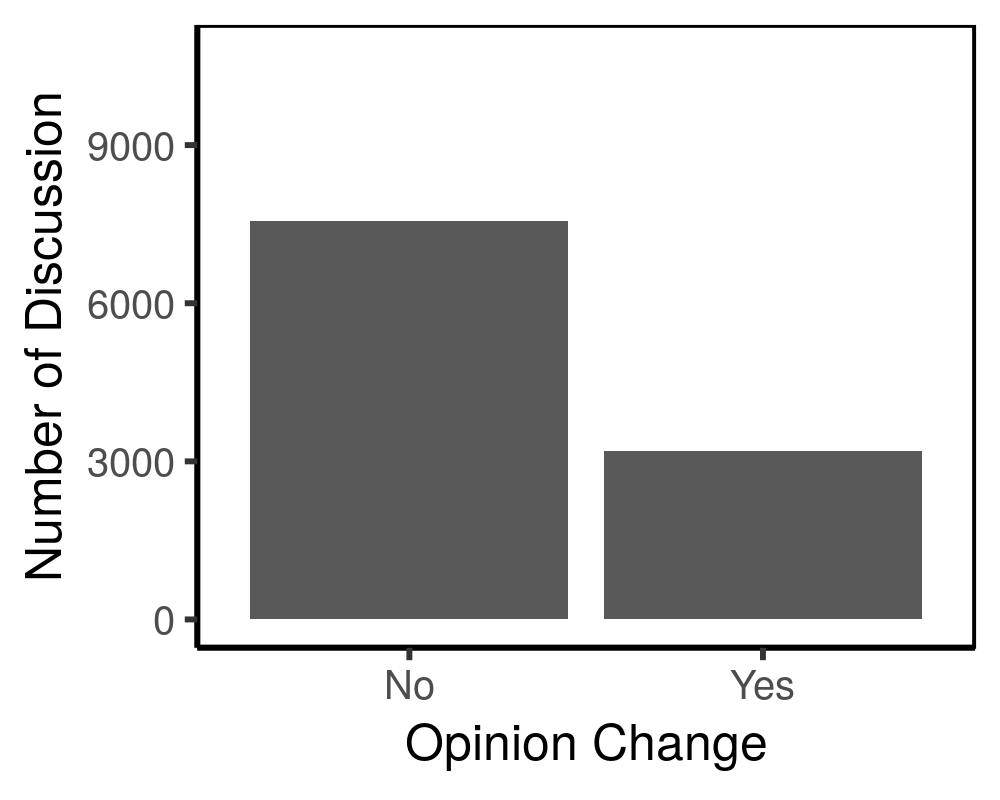
\includegraphics{../calc/fig/delta.png}}
\end{figure}
\end{frame}

\begin{frame}{Measuring Morality in Text}
\emph{Moral Foundations Dictionary:}\\
\footnotesize{(c.f., \citealt{graham2009liberals} and \url{http://www.moralfoundations.org/})}\\
\vspace{2em}
\begin{itemize}
	\item \emph{Care}: caring, compassion*, empath*, preserve, protect*, ...
	\item \emph{Fairness}: equal*, honest*, impartial*, justice, favoritism, ...
	\item \emph{Loyalty}: collectiv*, communal, family, homeland*, unite*, ...
	\item \emph{Authority}: command, comply, duty, hierarch*, honor*, ...
	\item \emph{Sanctity}: abstention, clean*, decen*, holy, innocent, ...
	\item \emph{General Morality}: character, commendable, decen*, ethic*, moral*, ...
\end{itemize}
\end{frame}

\begin{frame}{Moral Foundations and Persuadability}
\begin{figure}
	\only<1>{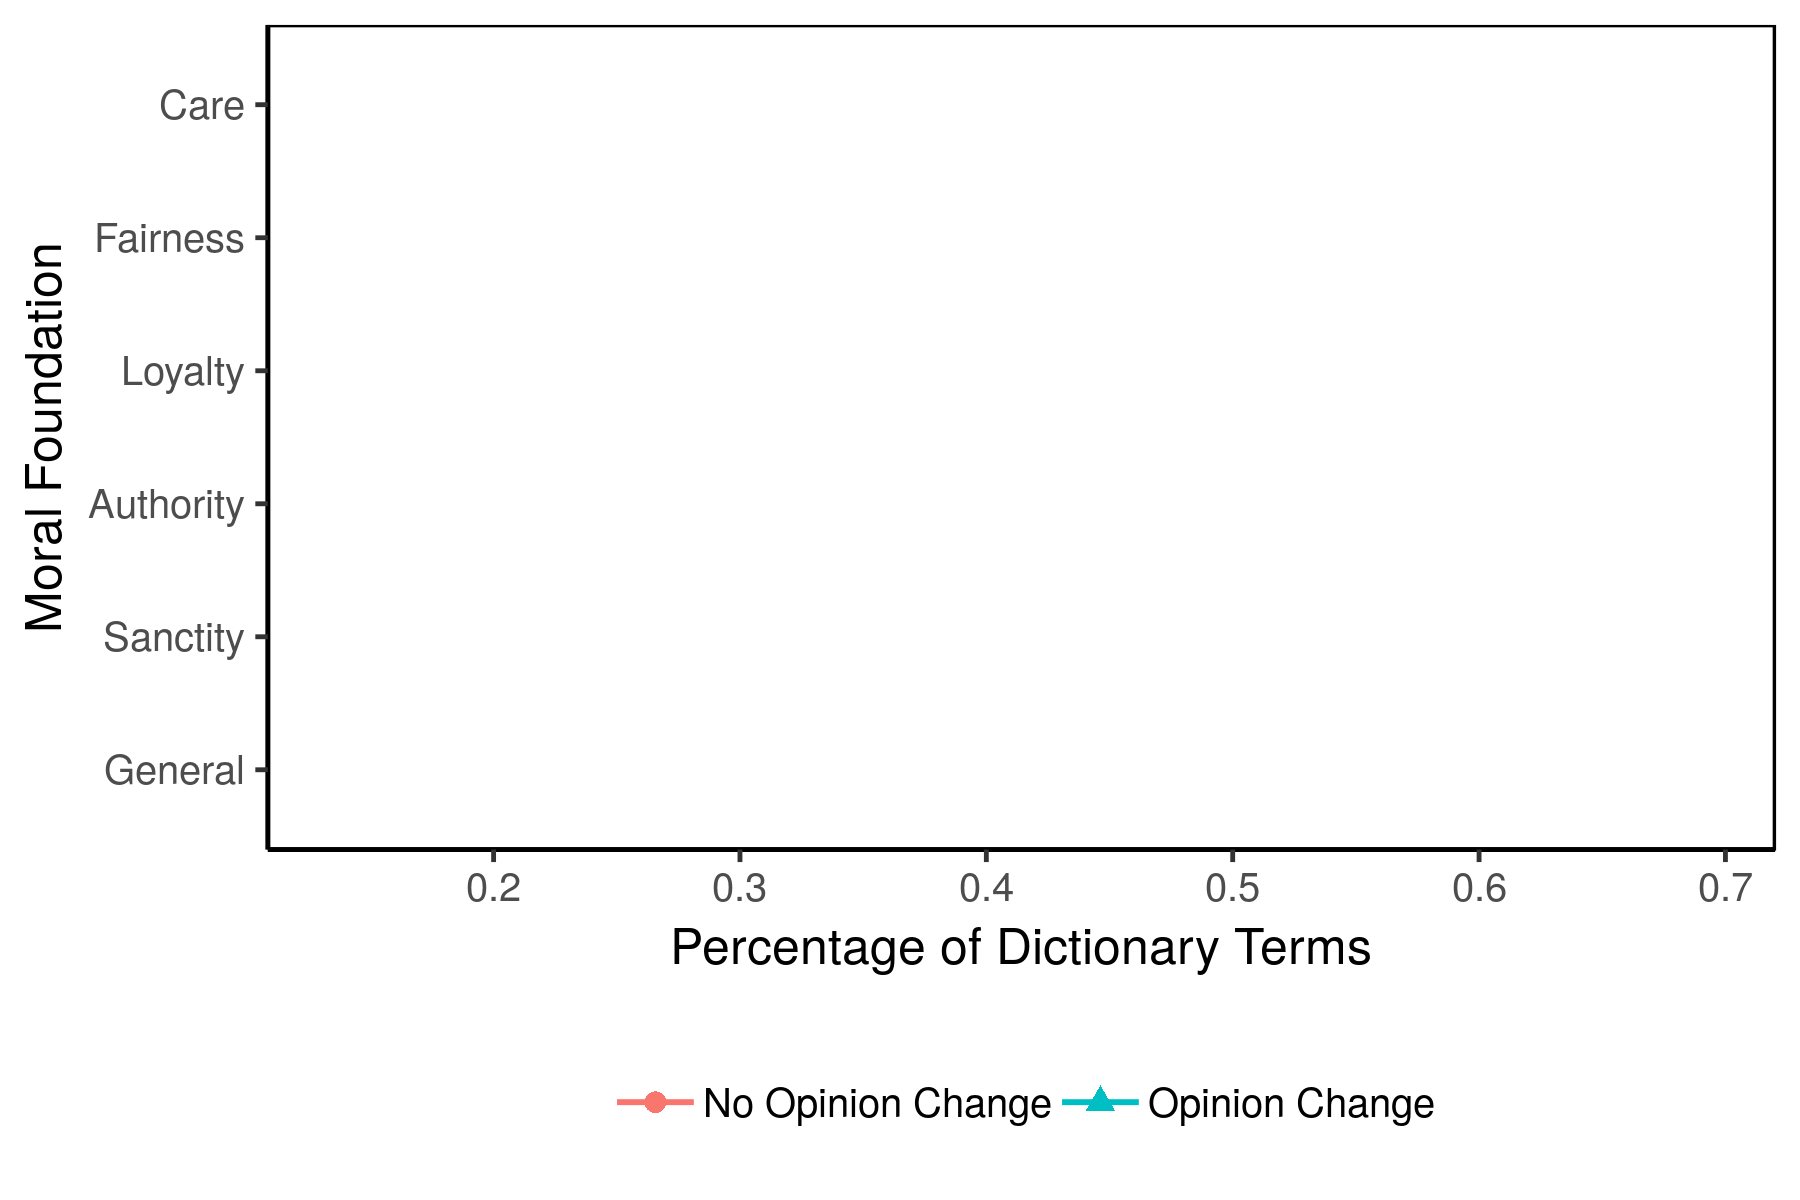
\includegraphics{../calc/fig/persuadability_empty.png}}\only<2>{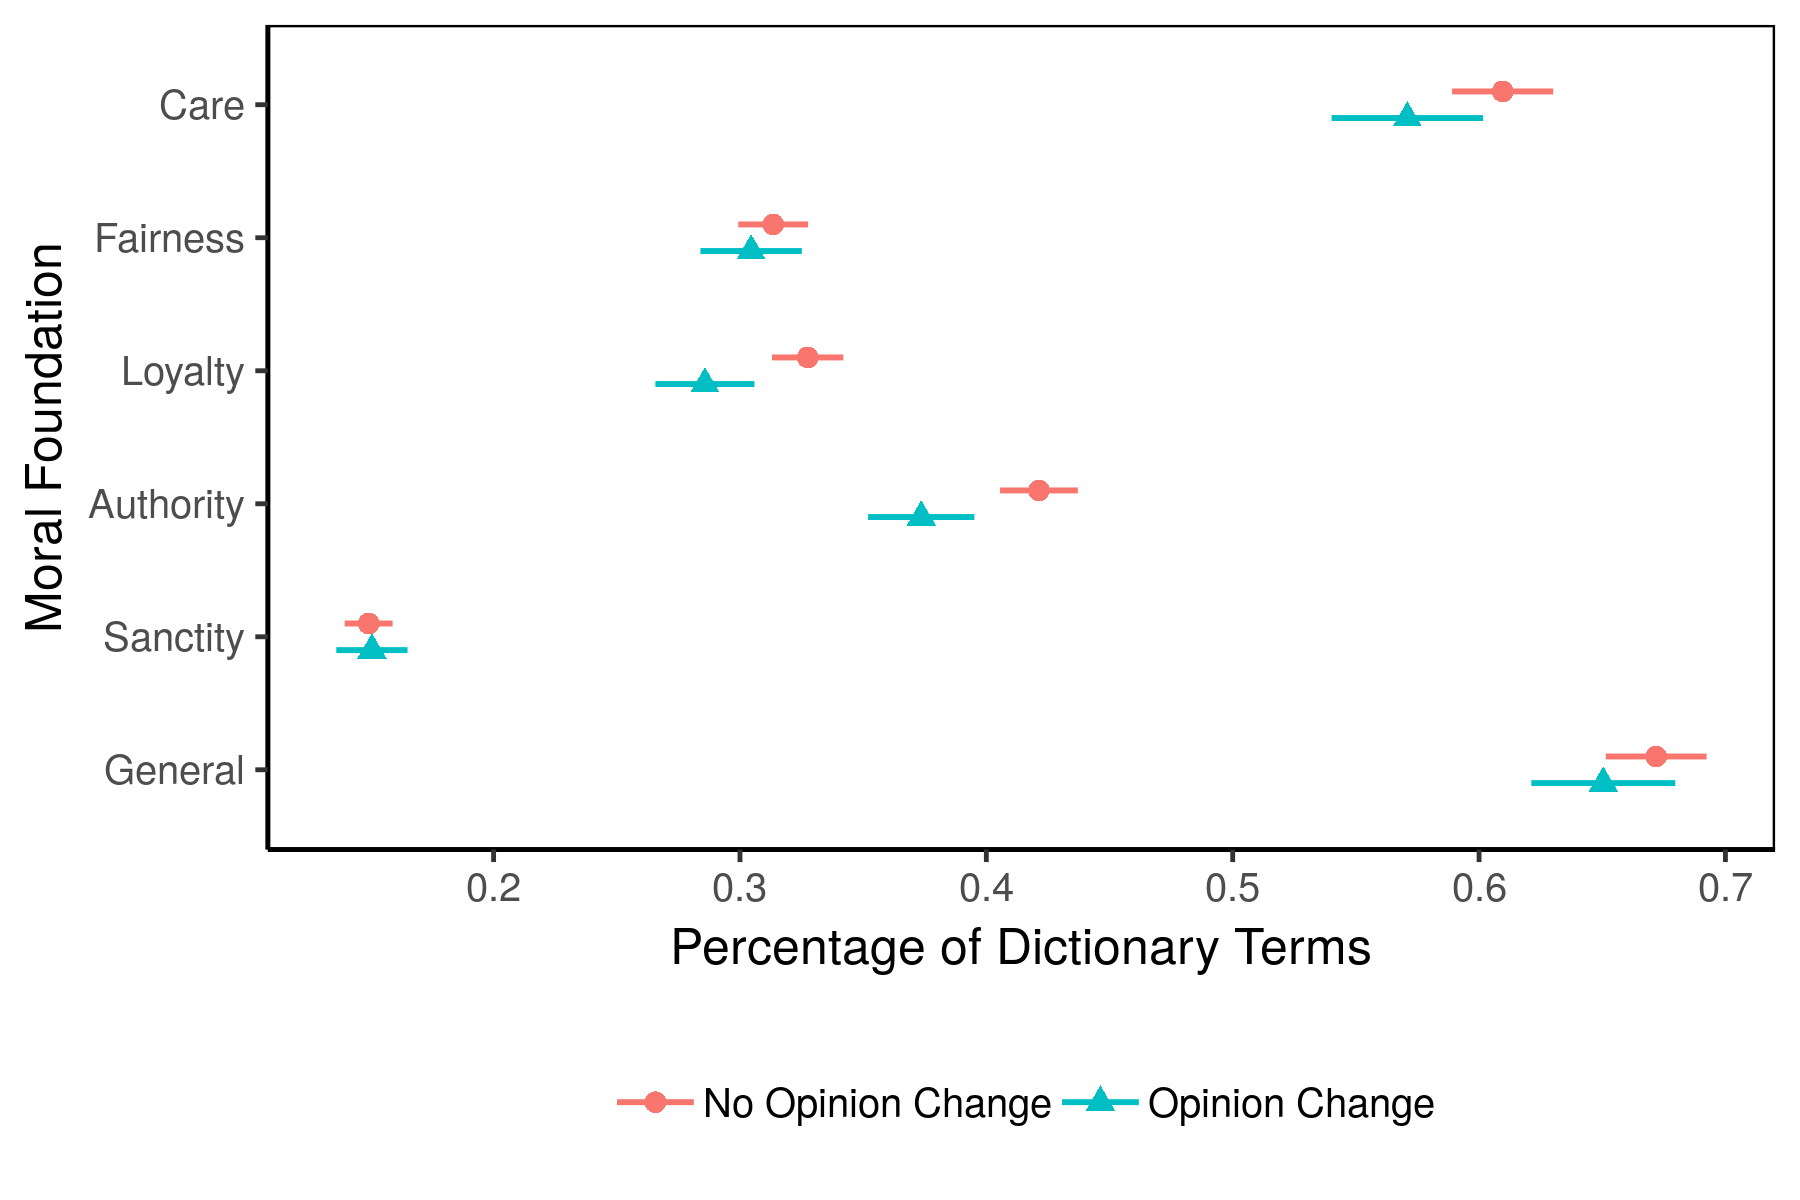
\includegraphics{../calc/fig/persuadability.png}}
\end{figure}
\end{frame}

\subsection{Counterarguments and Persuasiveness}
\begin{frame}{Exploring the Persuasiveness of Counterarguments}
\begin{figure}
	\only<1>{
\includegraphics[width=\textwidth]{fig/reddit-05.png}}
	\only<2>{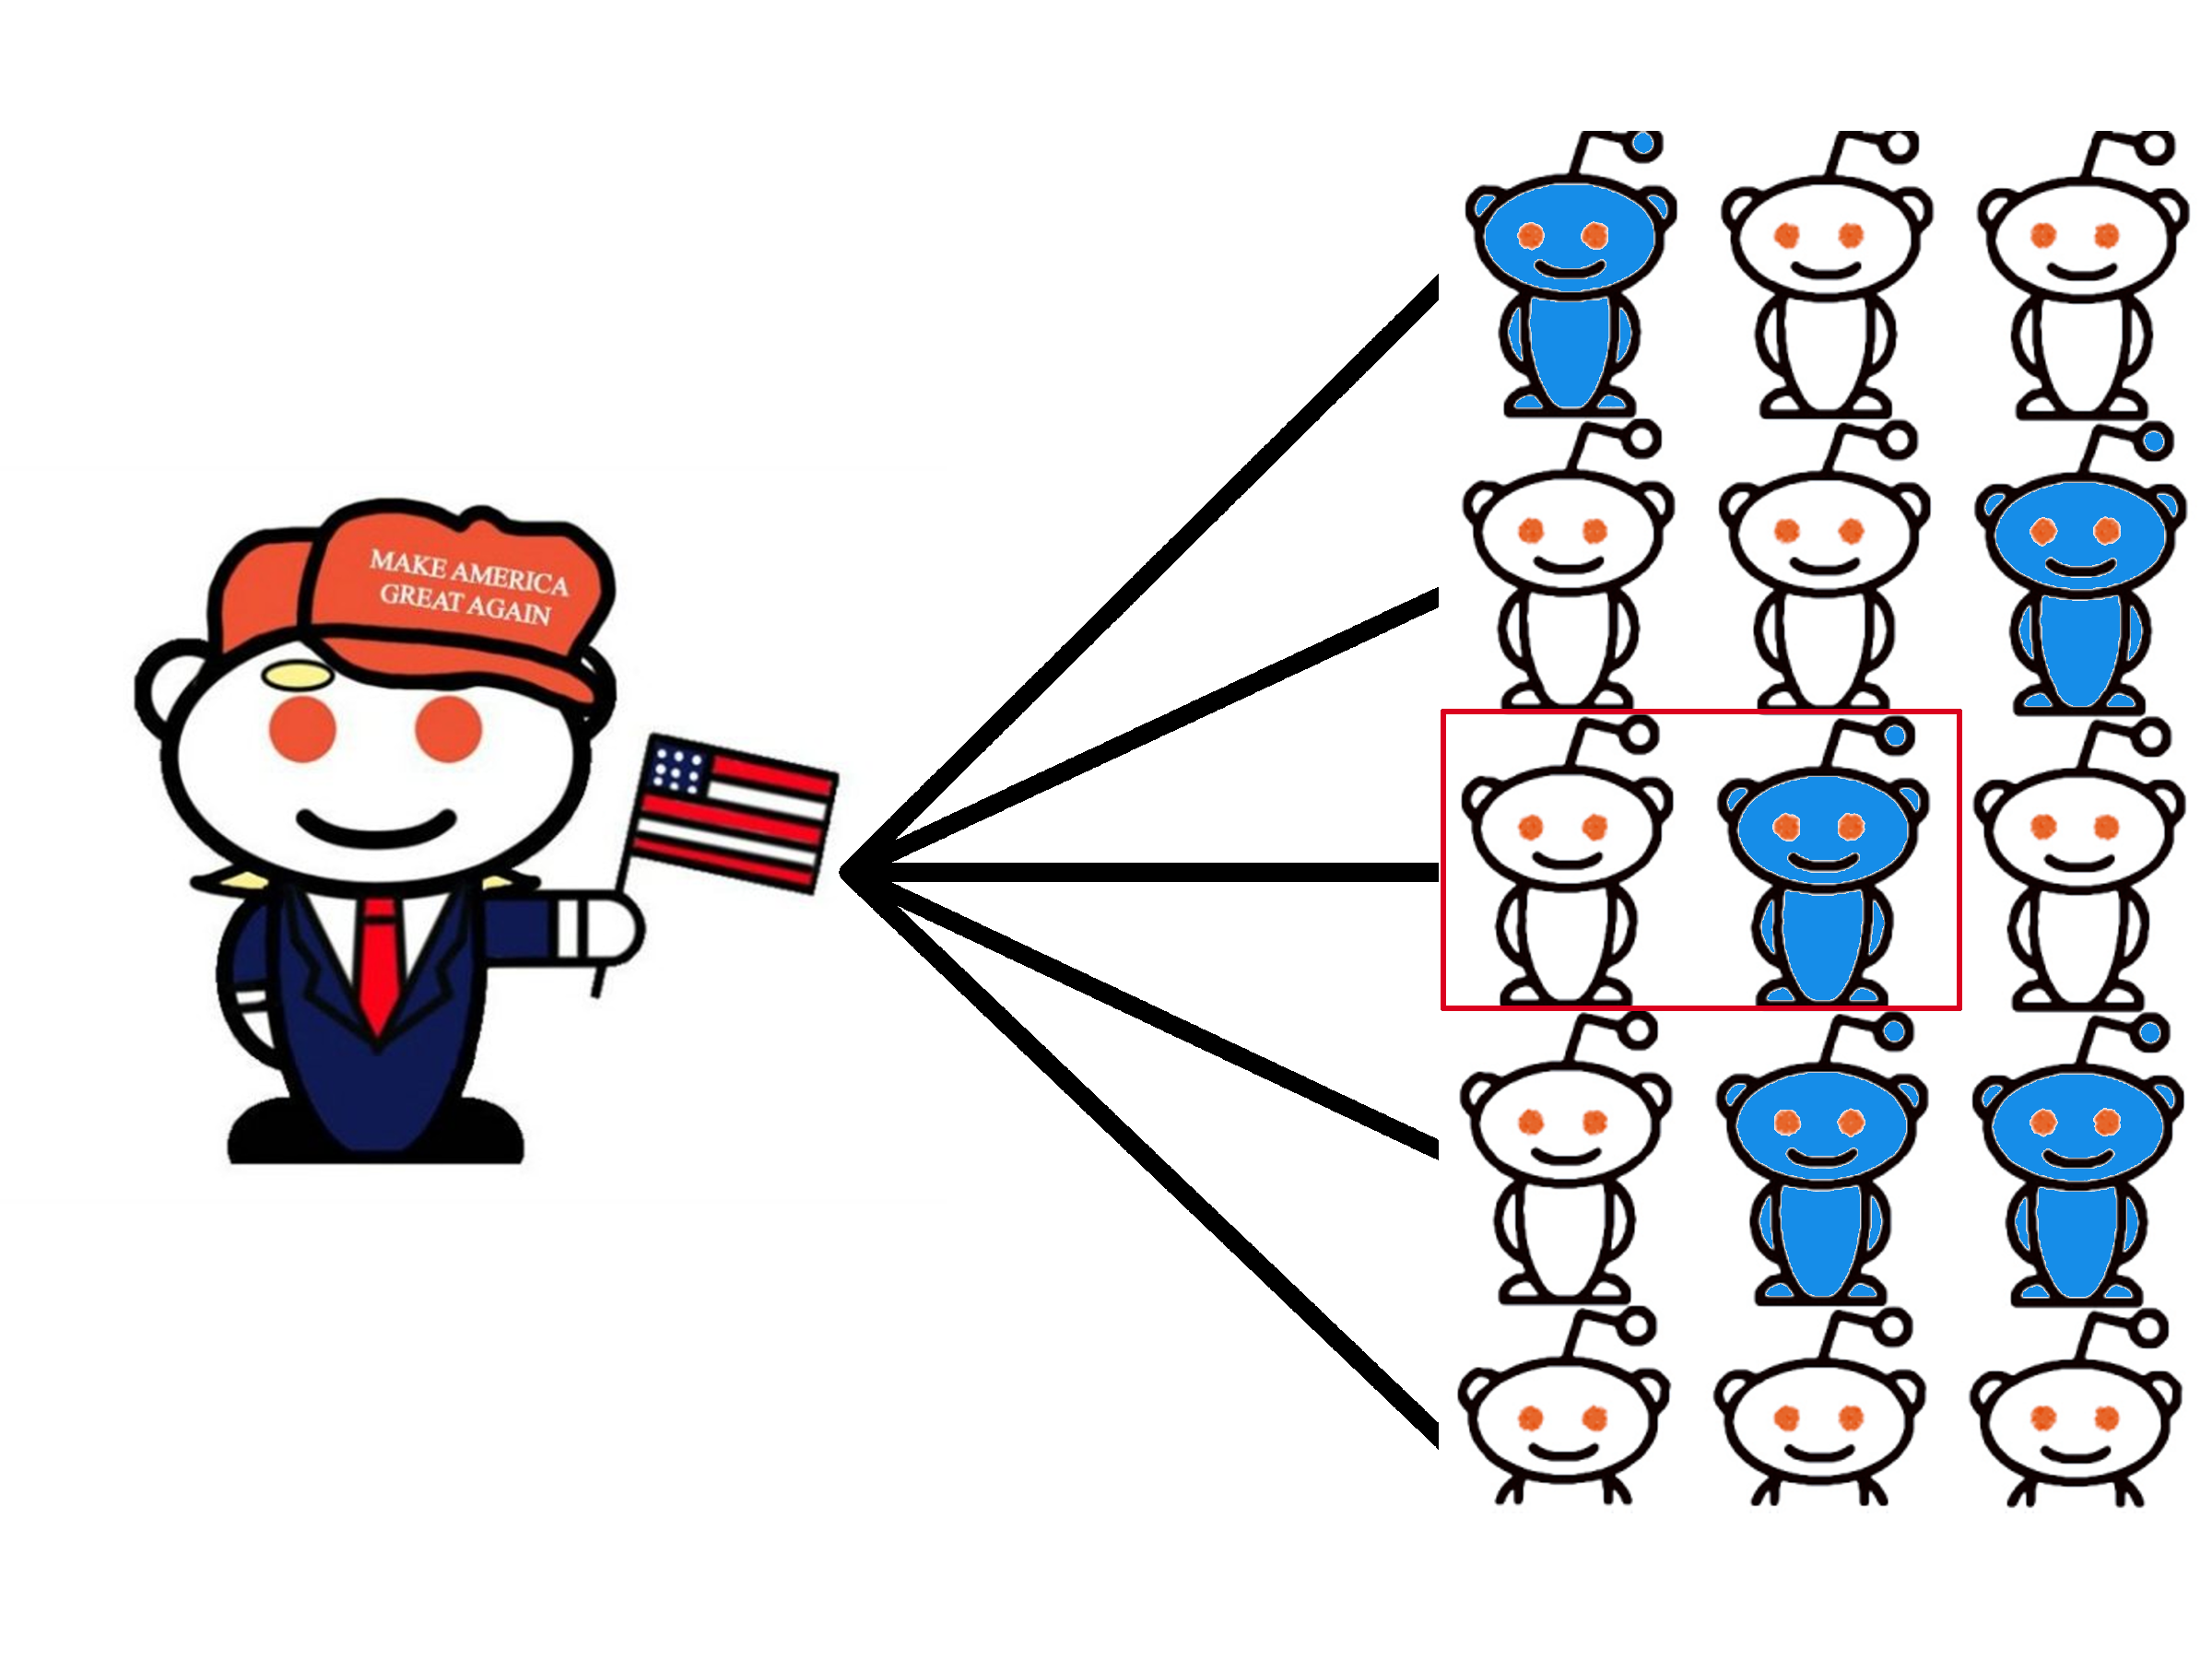
\includegraphics[width=\textwidth]{fig/reddit-06.png}}
\end{figure}
\end{frame}

\begin{frame}{Matching Similar Arguments}\centering
\begin{equation*}
\text{Jaccard}(B_\Delta,B_{\neg\Delta})=\dfrac{|B_\Delta\cap B_{\neg\Delta}|}{|B_\Delta\cup B_{\neg\Delta}|}
\end{equation*}
\vspace{2em}\\
\large{\emph{Question:}\\Which of two lexically similar arguments is the successful one?}
\end{frame}

\begin{frame}{Moral Foundations and Persuasiveness}
\begin{figure}
	\only<1>{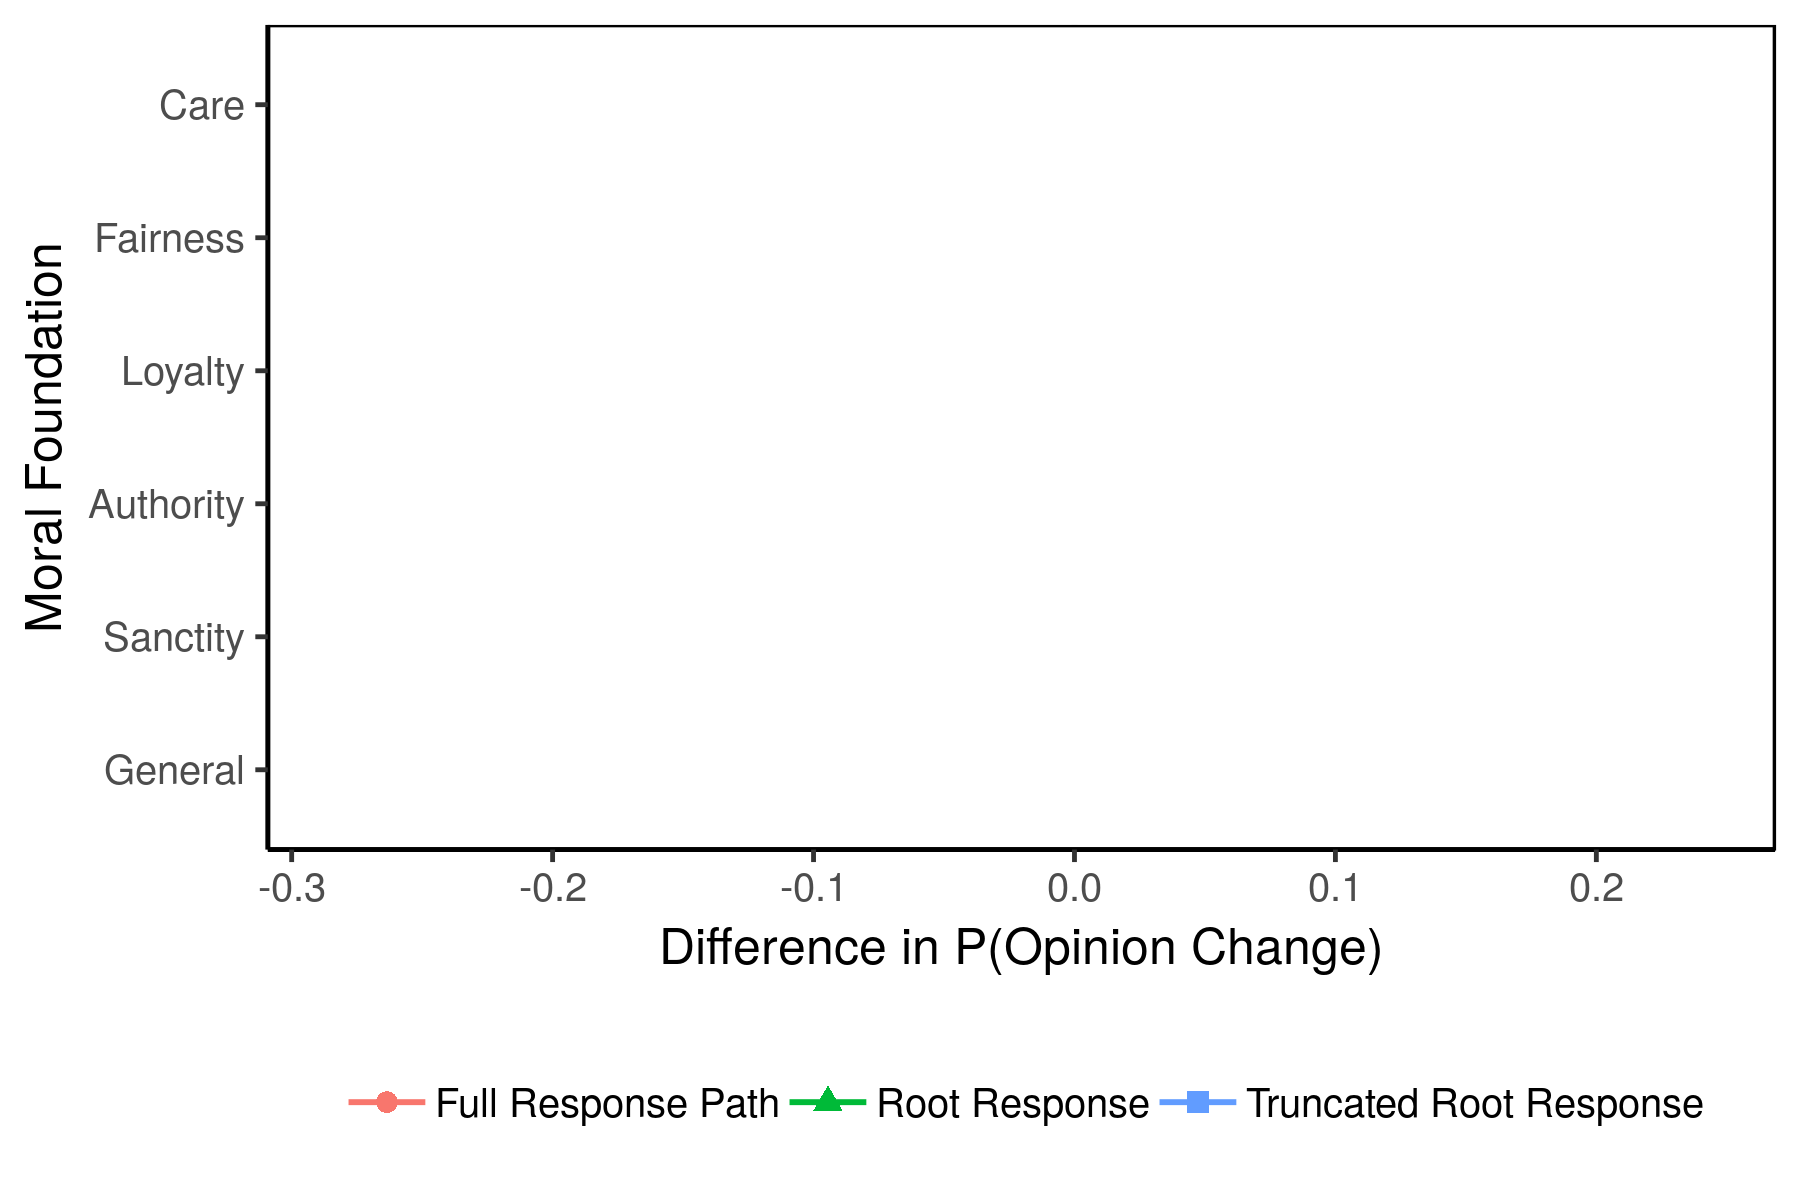
\includegraphics{../calc/fig/logit_persuasiveness_empty.png}}\only<2>{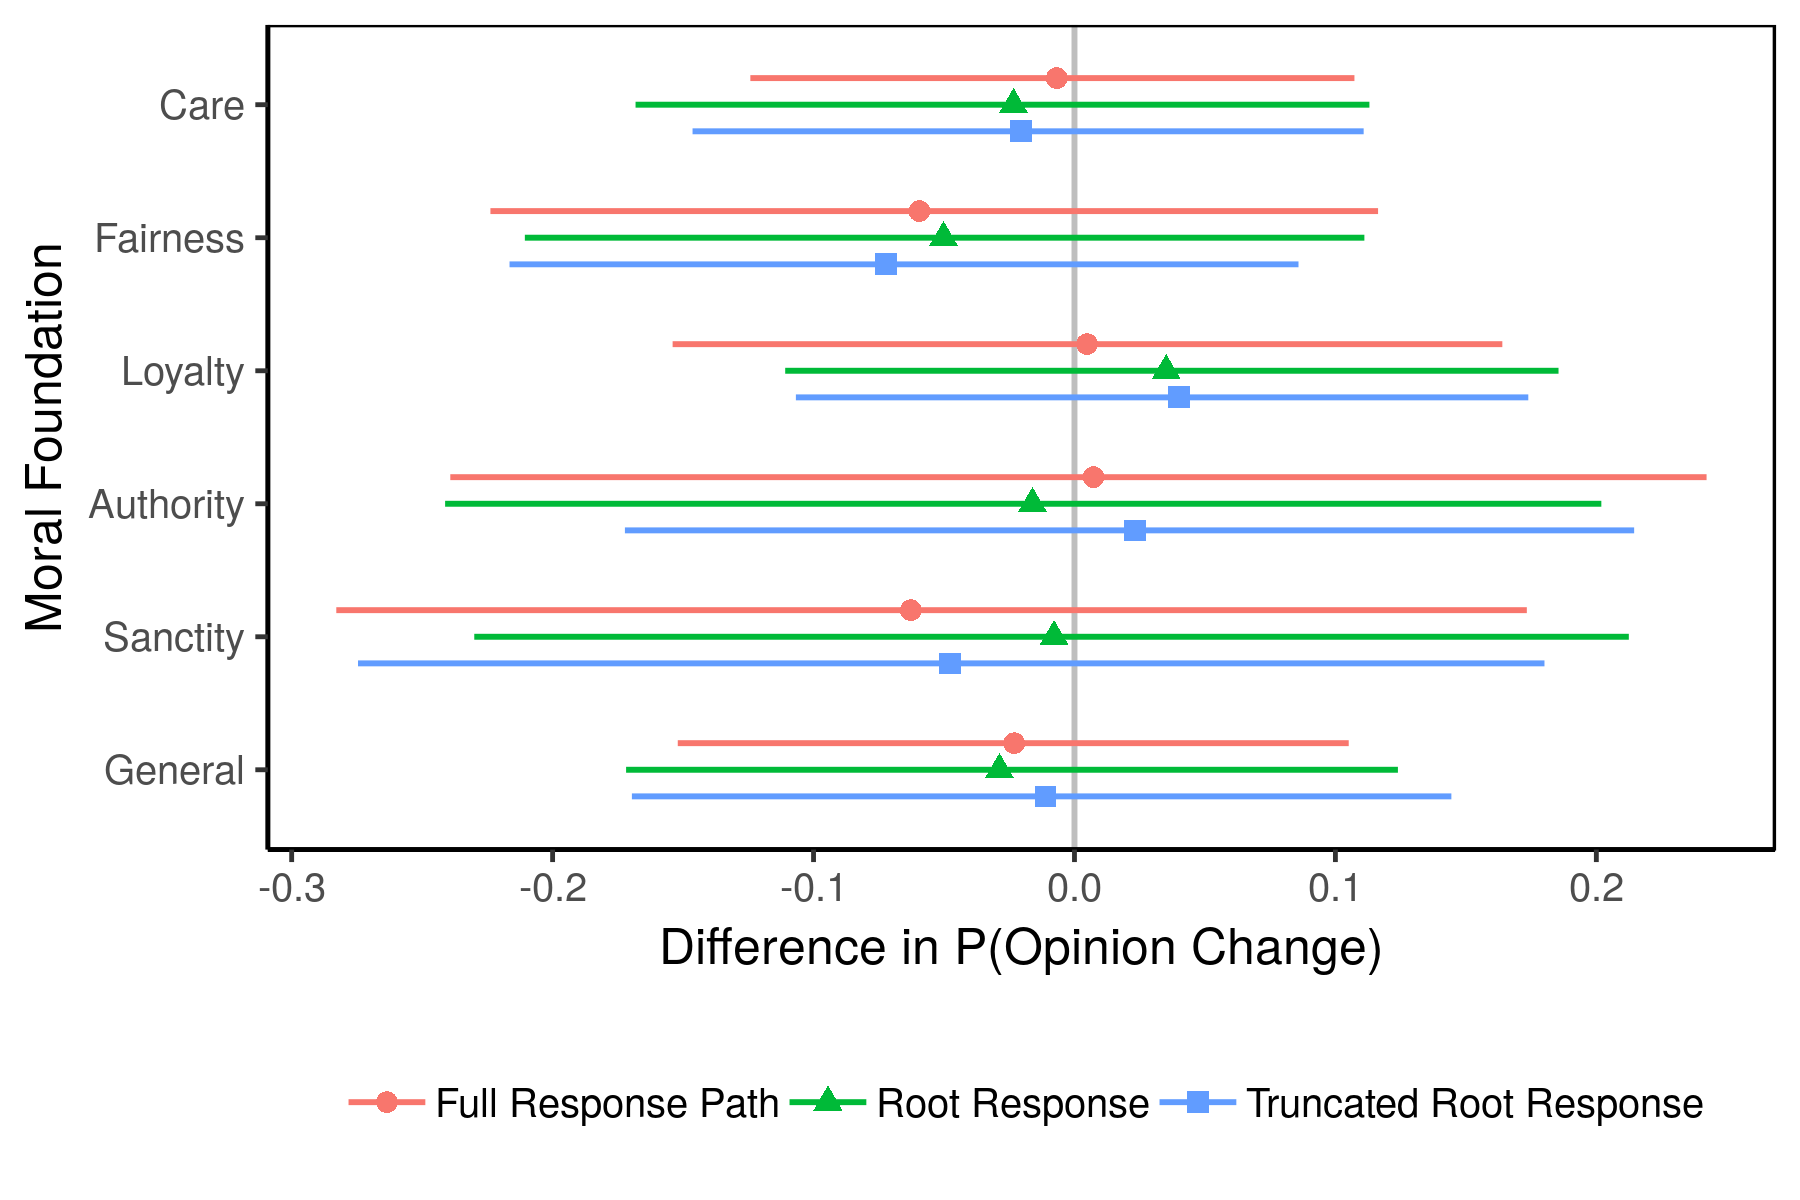
\includegraphics{../calc/fig/logit_persuasiveness.png}}
\end{figure}
\end{frame}

\begin{frame}{Measuring Moral Congruence}\centering
\begin{equation*}
\text{MFT Congruence}=\dfrac{\vec{a}\cdot \vec{b}}{||\vec{a}||\hspace{.2em}||\vec{b}||}
\end{equation*}
\vspace{2em}\\
\large{\emph{Basic Approach:}\\Measure the cosine similarity in dictionary counts between opening statements and counterarguments}
\end{frame}

\begin{frame}{Measuring Moral Congruence}
\begin{figure}
	\only<1>{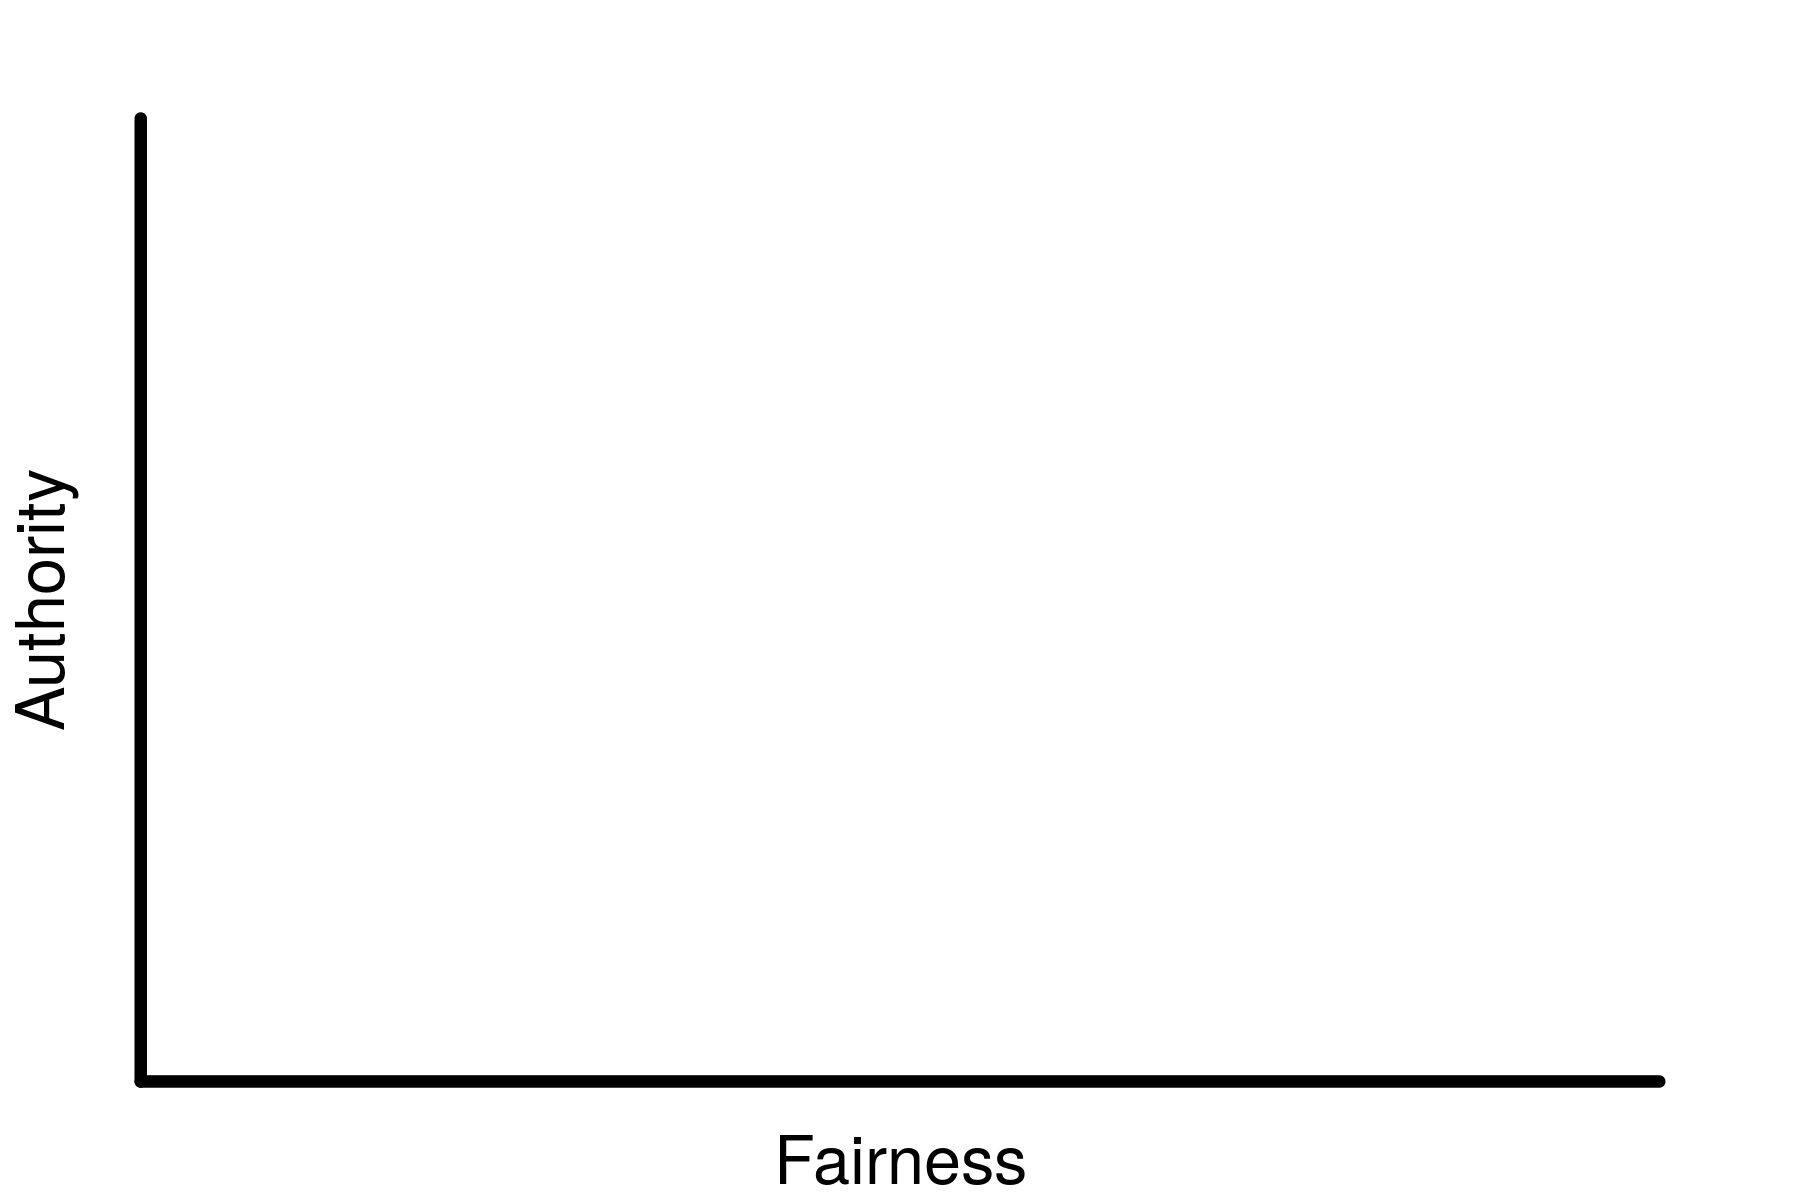
\includegraphics{../calc/fig/cosine_illu0.png}}\only<2>{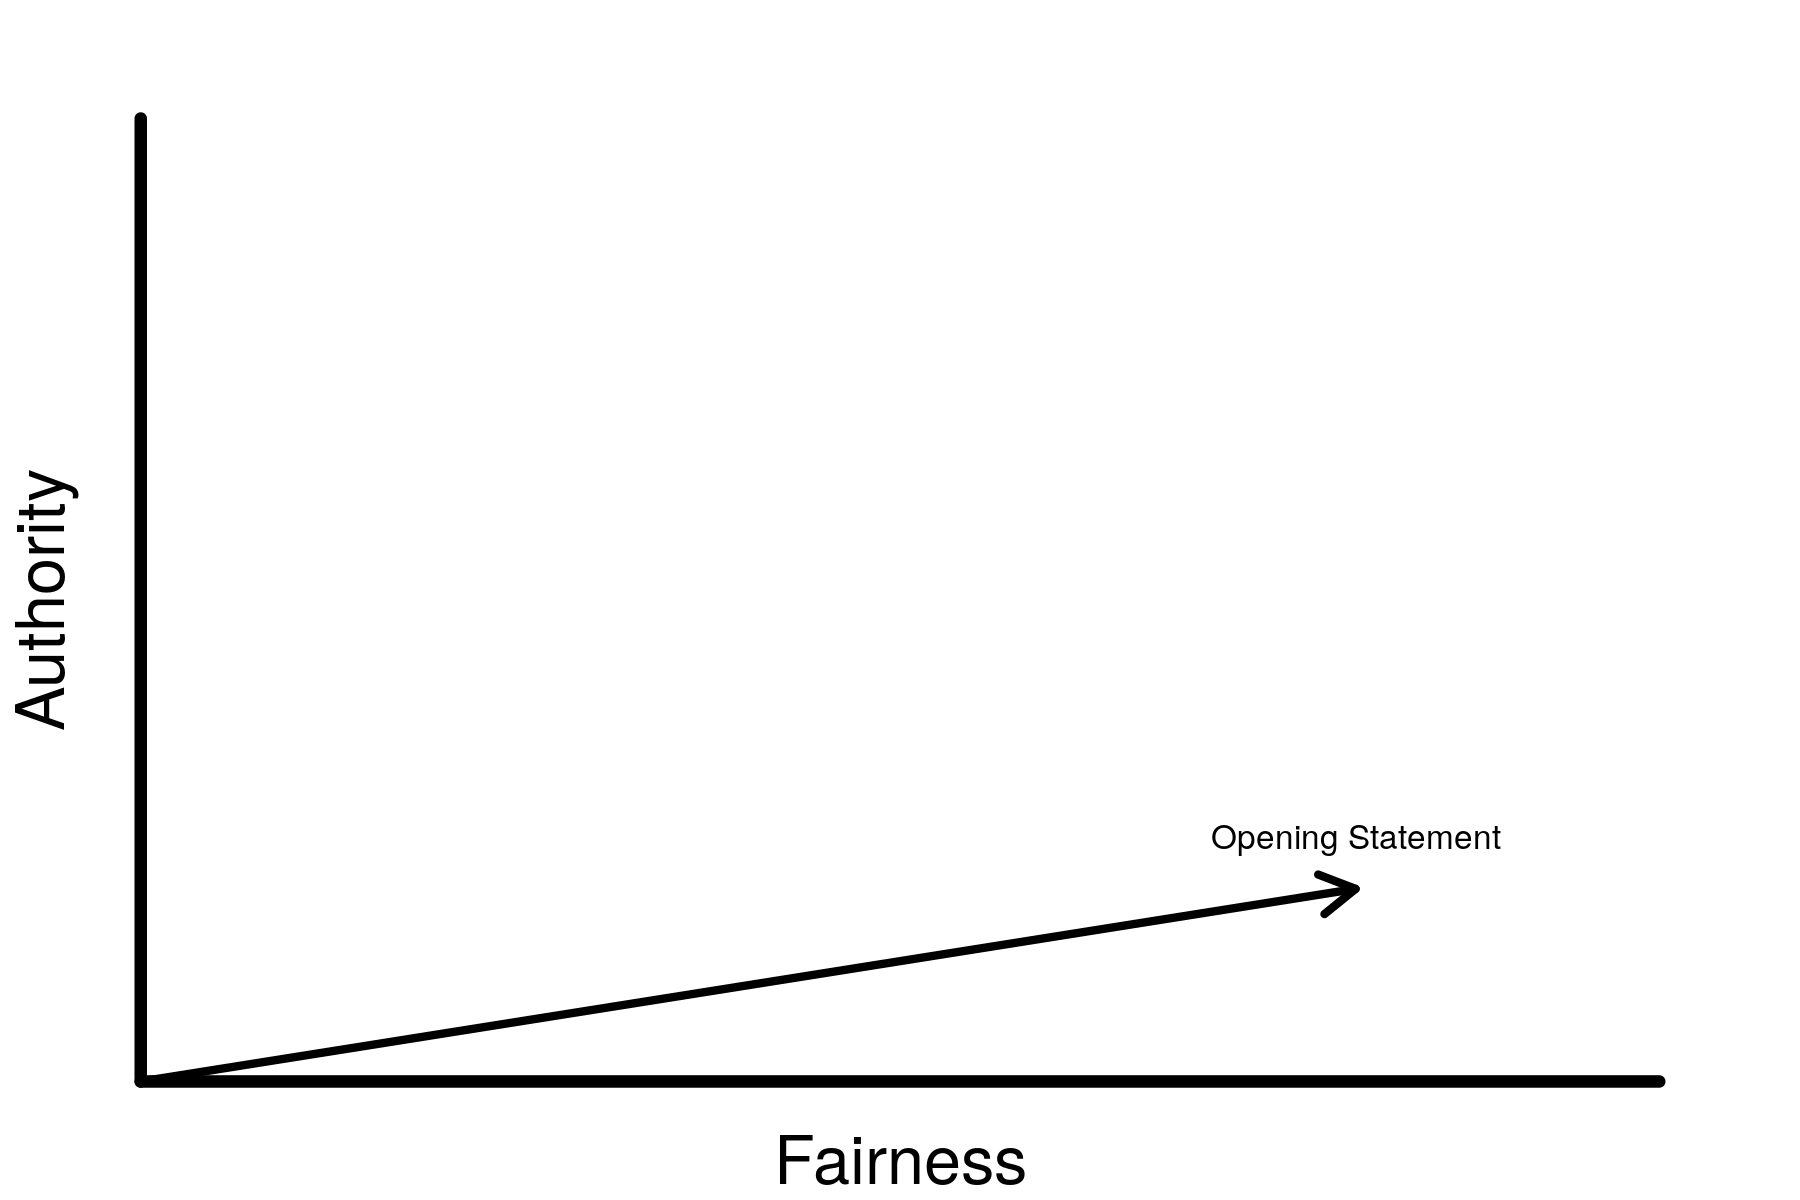
\includegraphics{../calc/fig/cosine_illu1.png}}\only<3>{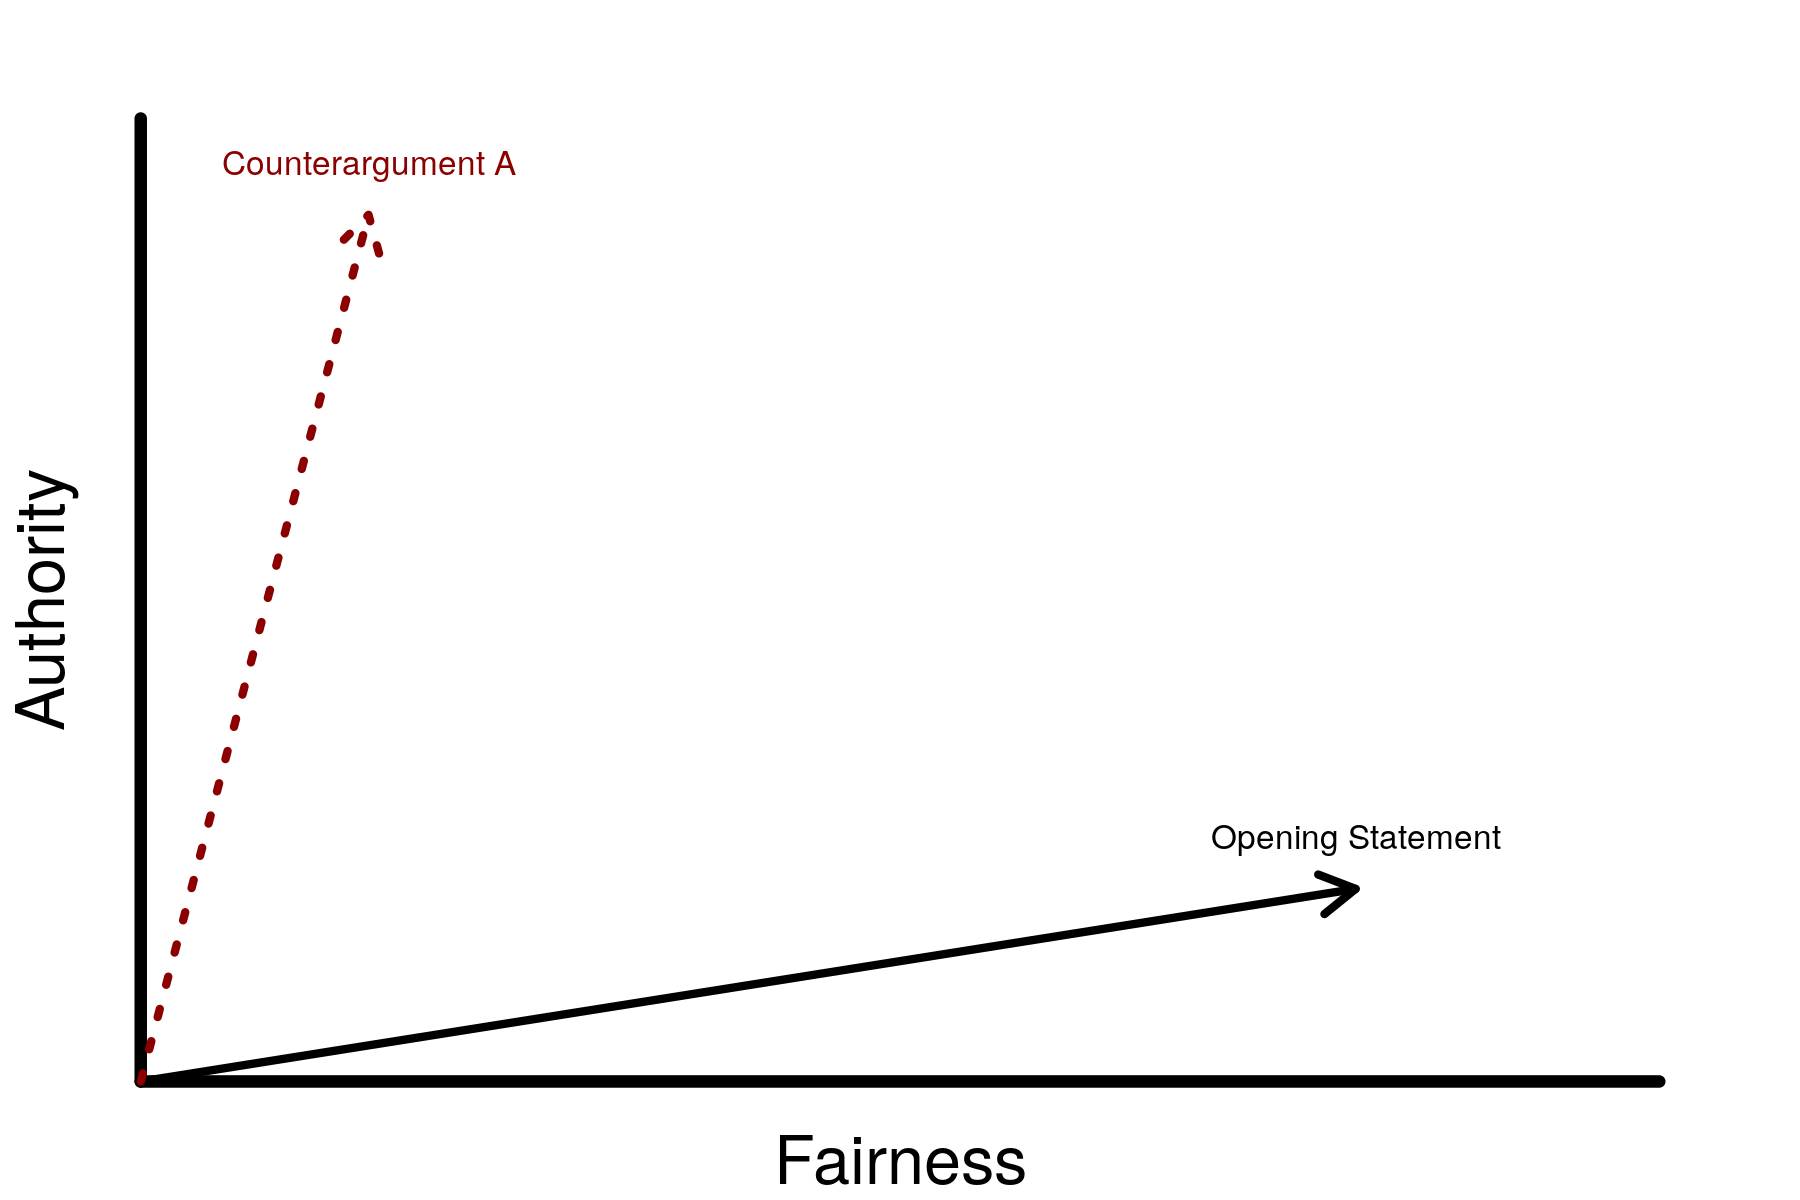
\includegraphics{../calc/fig/cosine_illu2.png}}\only<4>{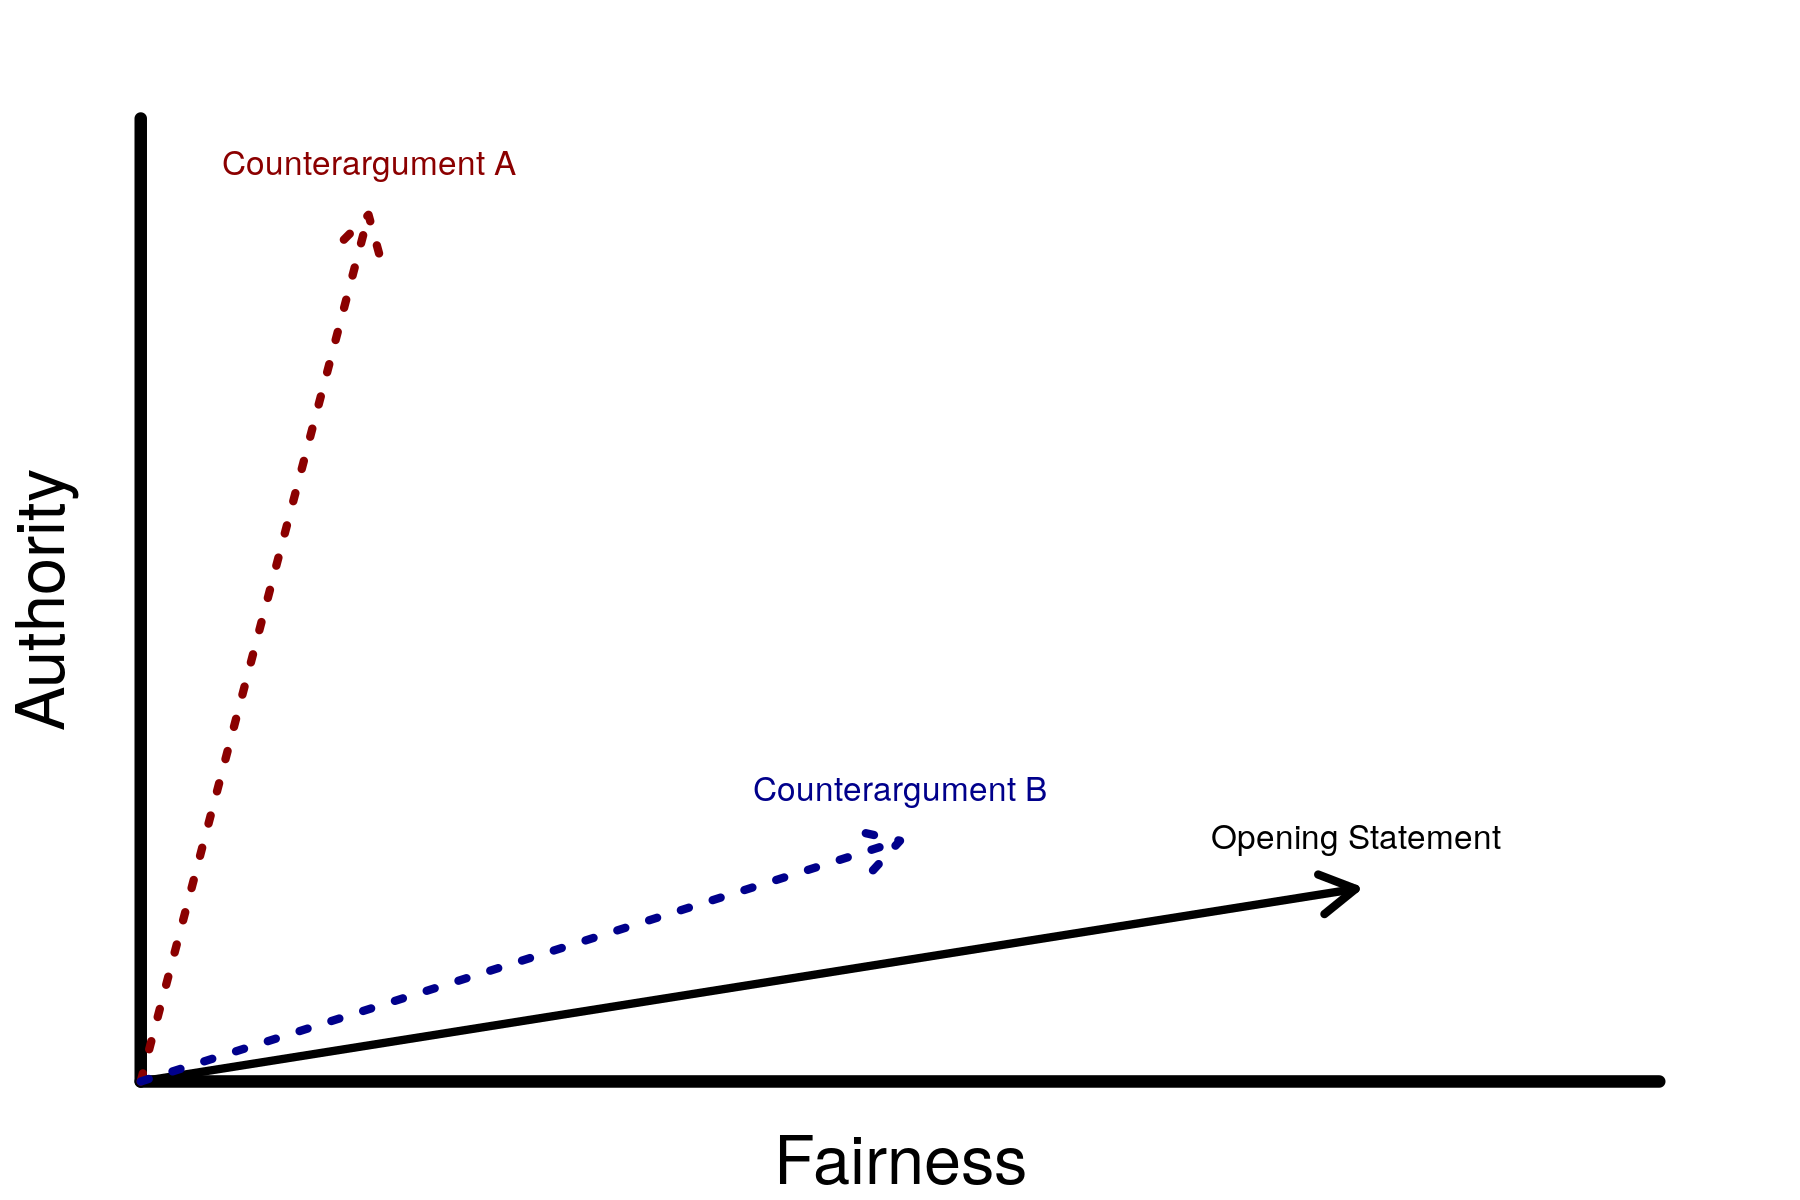
\includegraphics{../calc/fig/cosine_illu3.png}}
\end{figure}
\end{frame}

\begin{frame}{Moral Congruence and Persuasiveness}\centering
\begin{figure}
\only<1>{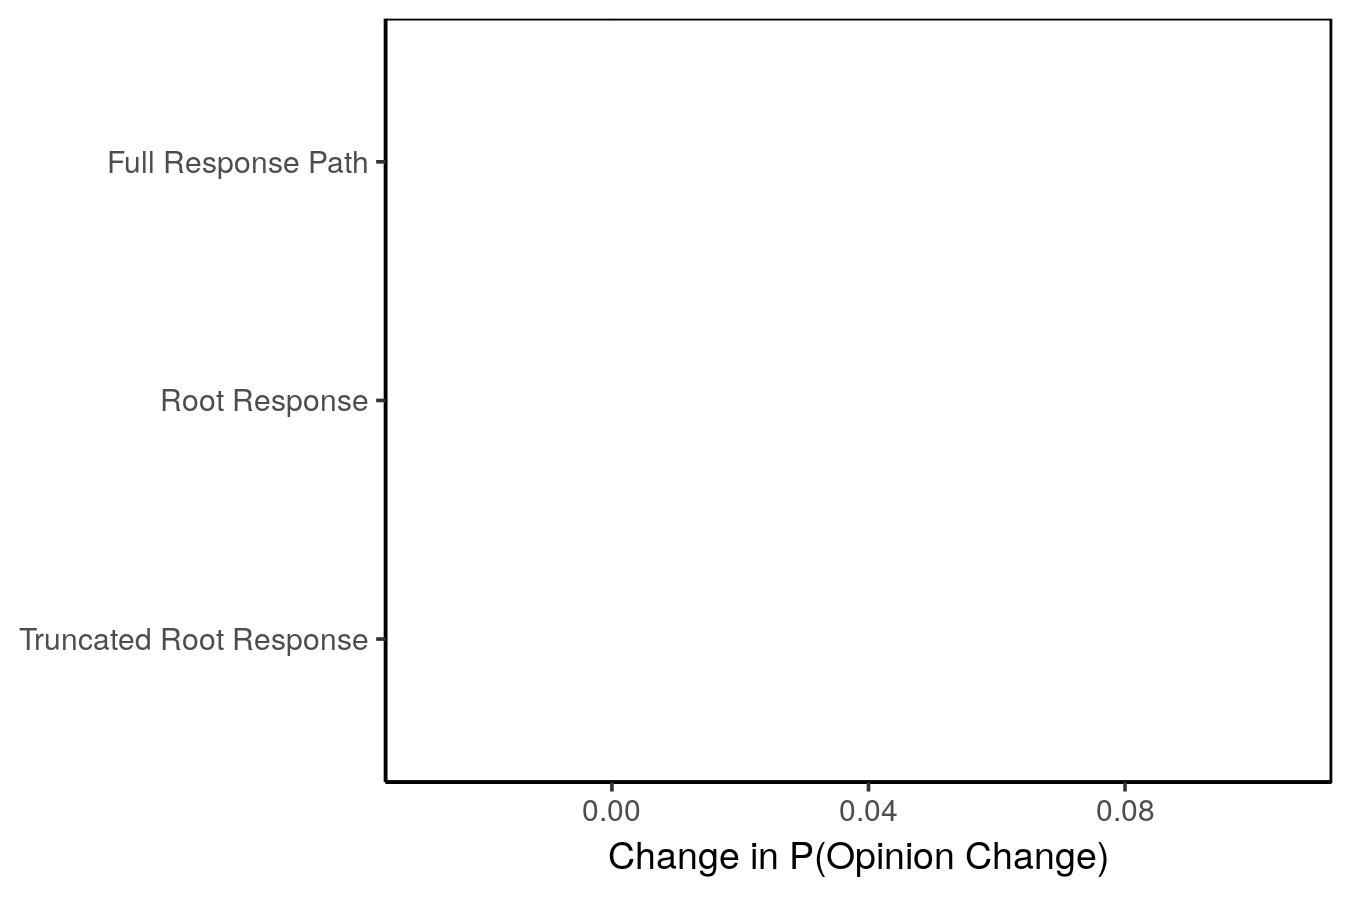
\includegraphics{../calc/fig/logit_cosine_empty.png}}\only<2>{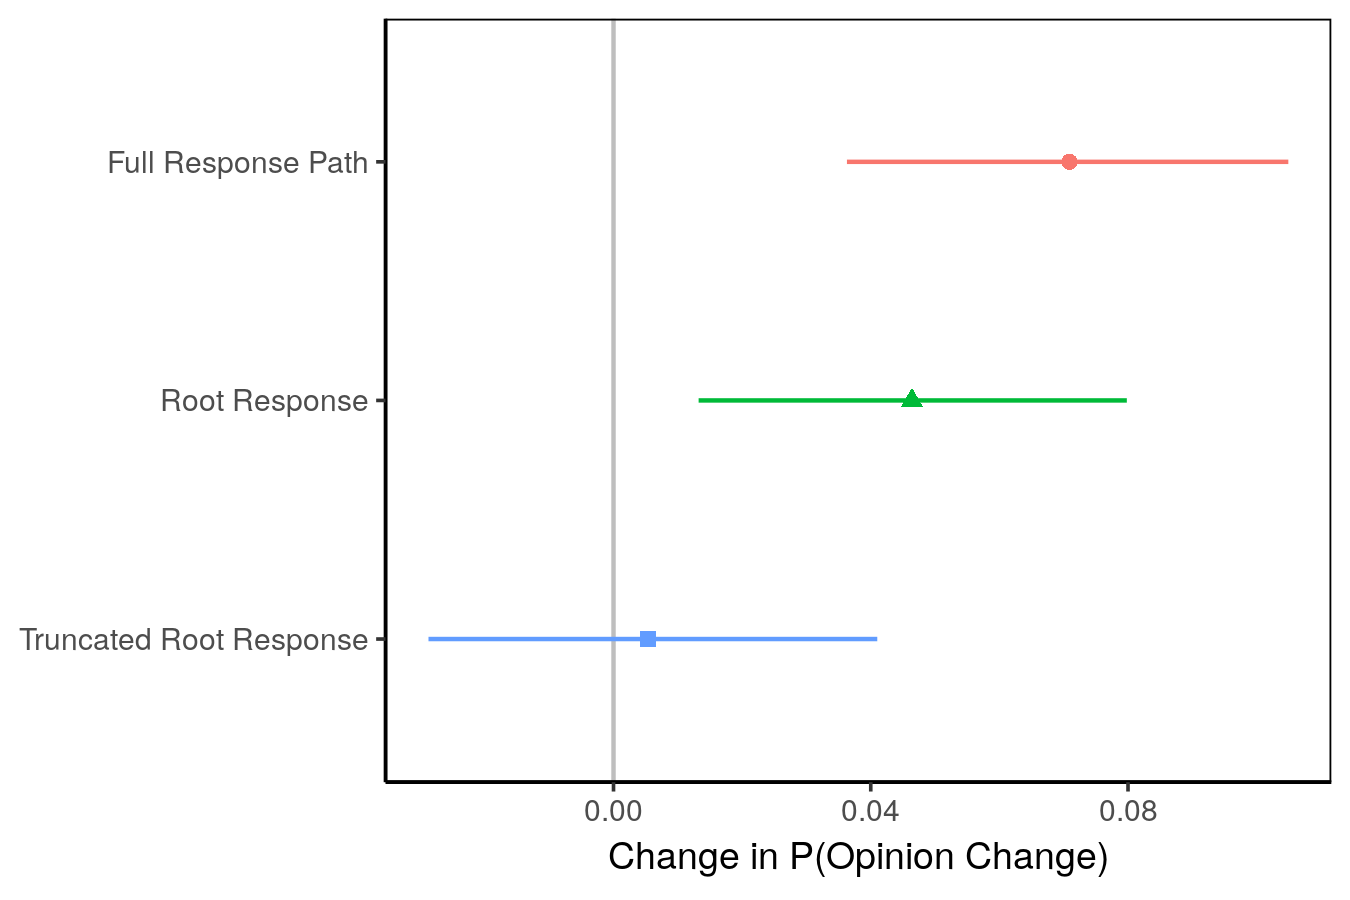
\includegraphics{../calc/fig/logit_cosine.png}}
\end{figure}
\end{frame}


\section{Conclusion}

\begin{frame}{Conclusion -- Discussions, Disagreement, and Morality}
Two \emph{opposing} hypotheses:\\
\vspace{2em}
\begin{tabularx}{\textwidth}{lX}
	\textcolor<2>{lightgray}{\textcolor<1>{beamer@sbred}{Moral Conviction}:} & \textcolor<2>{lightgray}{Arguments that involve \textcolor<1>{beamer@sbred}{moral appeals} will be \textcolor<1>{beamer@sbred}{less persuasive} than arguments that do not involve moral appeals.}\\
	& \\
	\emph{Moral Foundations}: & Arguments that involve \emph{moral appeals} will be \emph{more persuasive} than arguments that do not involve moral appeals, but only if they are \emph{congruent} with the opening statement's moral framework.
\end{tabularx}
\\\vspace{2em}
\uncover<2>{\emph{$\Rightarrow$ Moral appeals are futile unless we're speaking the same moral language}}
\end{frame}

\begin{frame}{Future Directions}
\begin{itemize}
	\item Collect new data, extract additional information about individual users (other subreddits etc.)
	\item Survey users on \texttt{/r/ChangeMyView}
	\item Experimental manipulation of opening statements
	\item Discussions in the lab
	\item \textbf{\emph{...}}
\end{itemize}
\end{frame}

\begin{frame}%[allowframebreaks]
\begin{columns}
	\begin{column}{.6\textwidth}
		\begin{center}
			{\Large \emph{Thank you for your attention!}}\\ \vspace{2em}
			Manuscript and code available at:\\
			\emph{\texttt{https://github.com/pwkraft/cmv}}\\ \vspace{2em}
			Comments, questions?\\
			\emph{\faEnvelopeO\hspace{.5em}\texttt{kraftp@uwm.edu}}\\\vspace{2em}
			\emph{\faGlobe\hspace{.5em}\texttt{pwkraft.github.io}}\\
			\emph{\faTwitter\hspace{.5em}\texttt{@patrickwkraft}}\\
		\end{center}
	\end{column}
	\begin{column}{.4\textwidth}
		\begin{figure}
			
\includegraphics[width=\textwidth]{fig/bad_opinions.png}
		\end{figure}
	\end{column}
\end{columns}

\end{frame}

\section*{Content}
\label{sec:main-content}
\begin{frame}%[allowframebreaks]
\frametitle{Content}
\tableofcontents %[hideallsubsections]
\end{frame}

\appendix
\section*{Appendix Content}
\label{sec:appendix-content}
\begin{frame}%[allowframebreaks]
\frametitle{Appendix Content}
\small\tableofcontents %[hideallsubsections]
\end{frame}

\section{Topic Differences and Persuadability}
\begin{frame}{Topic Differences and Persuadability}
\begin{figure}
	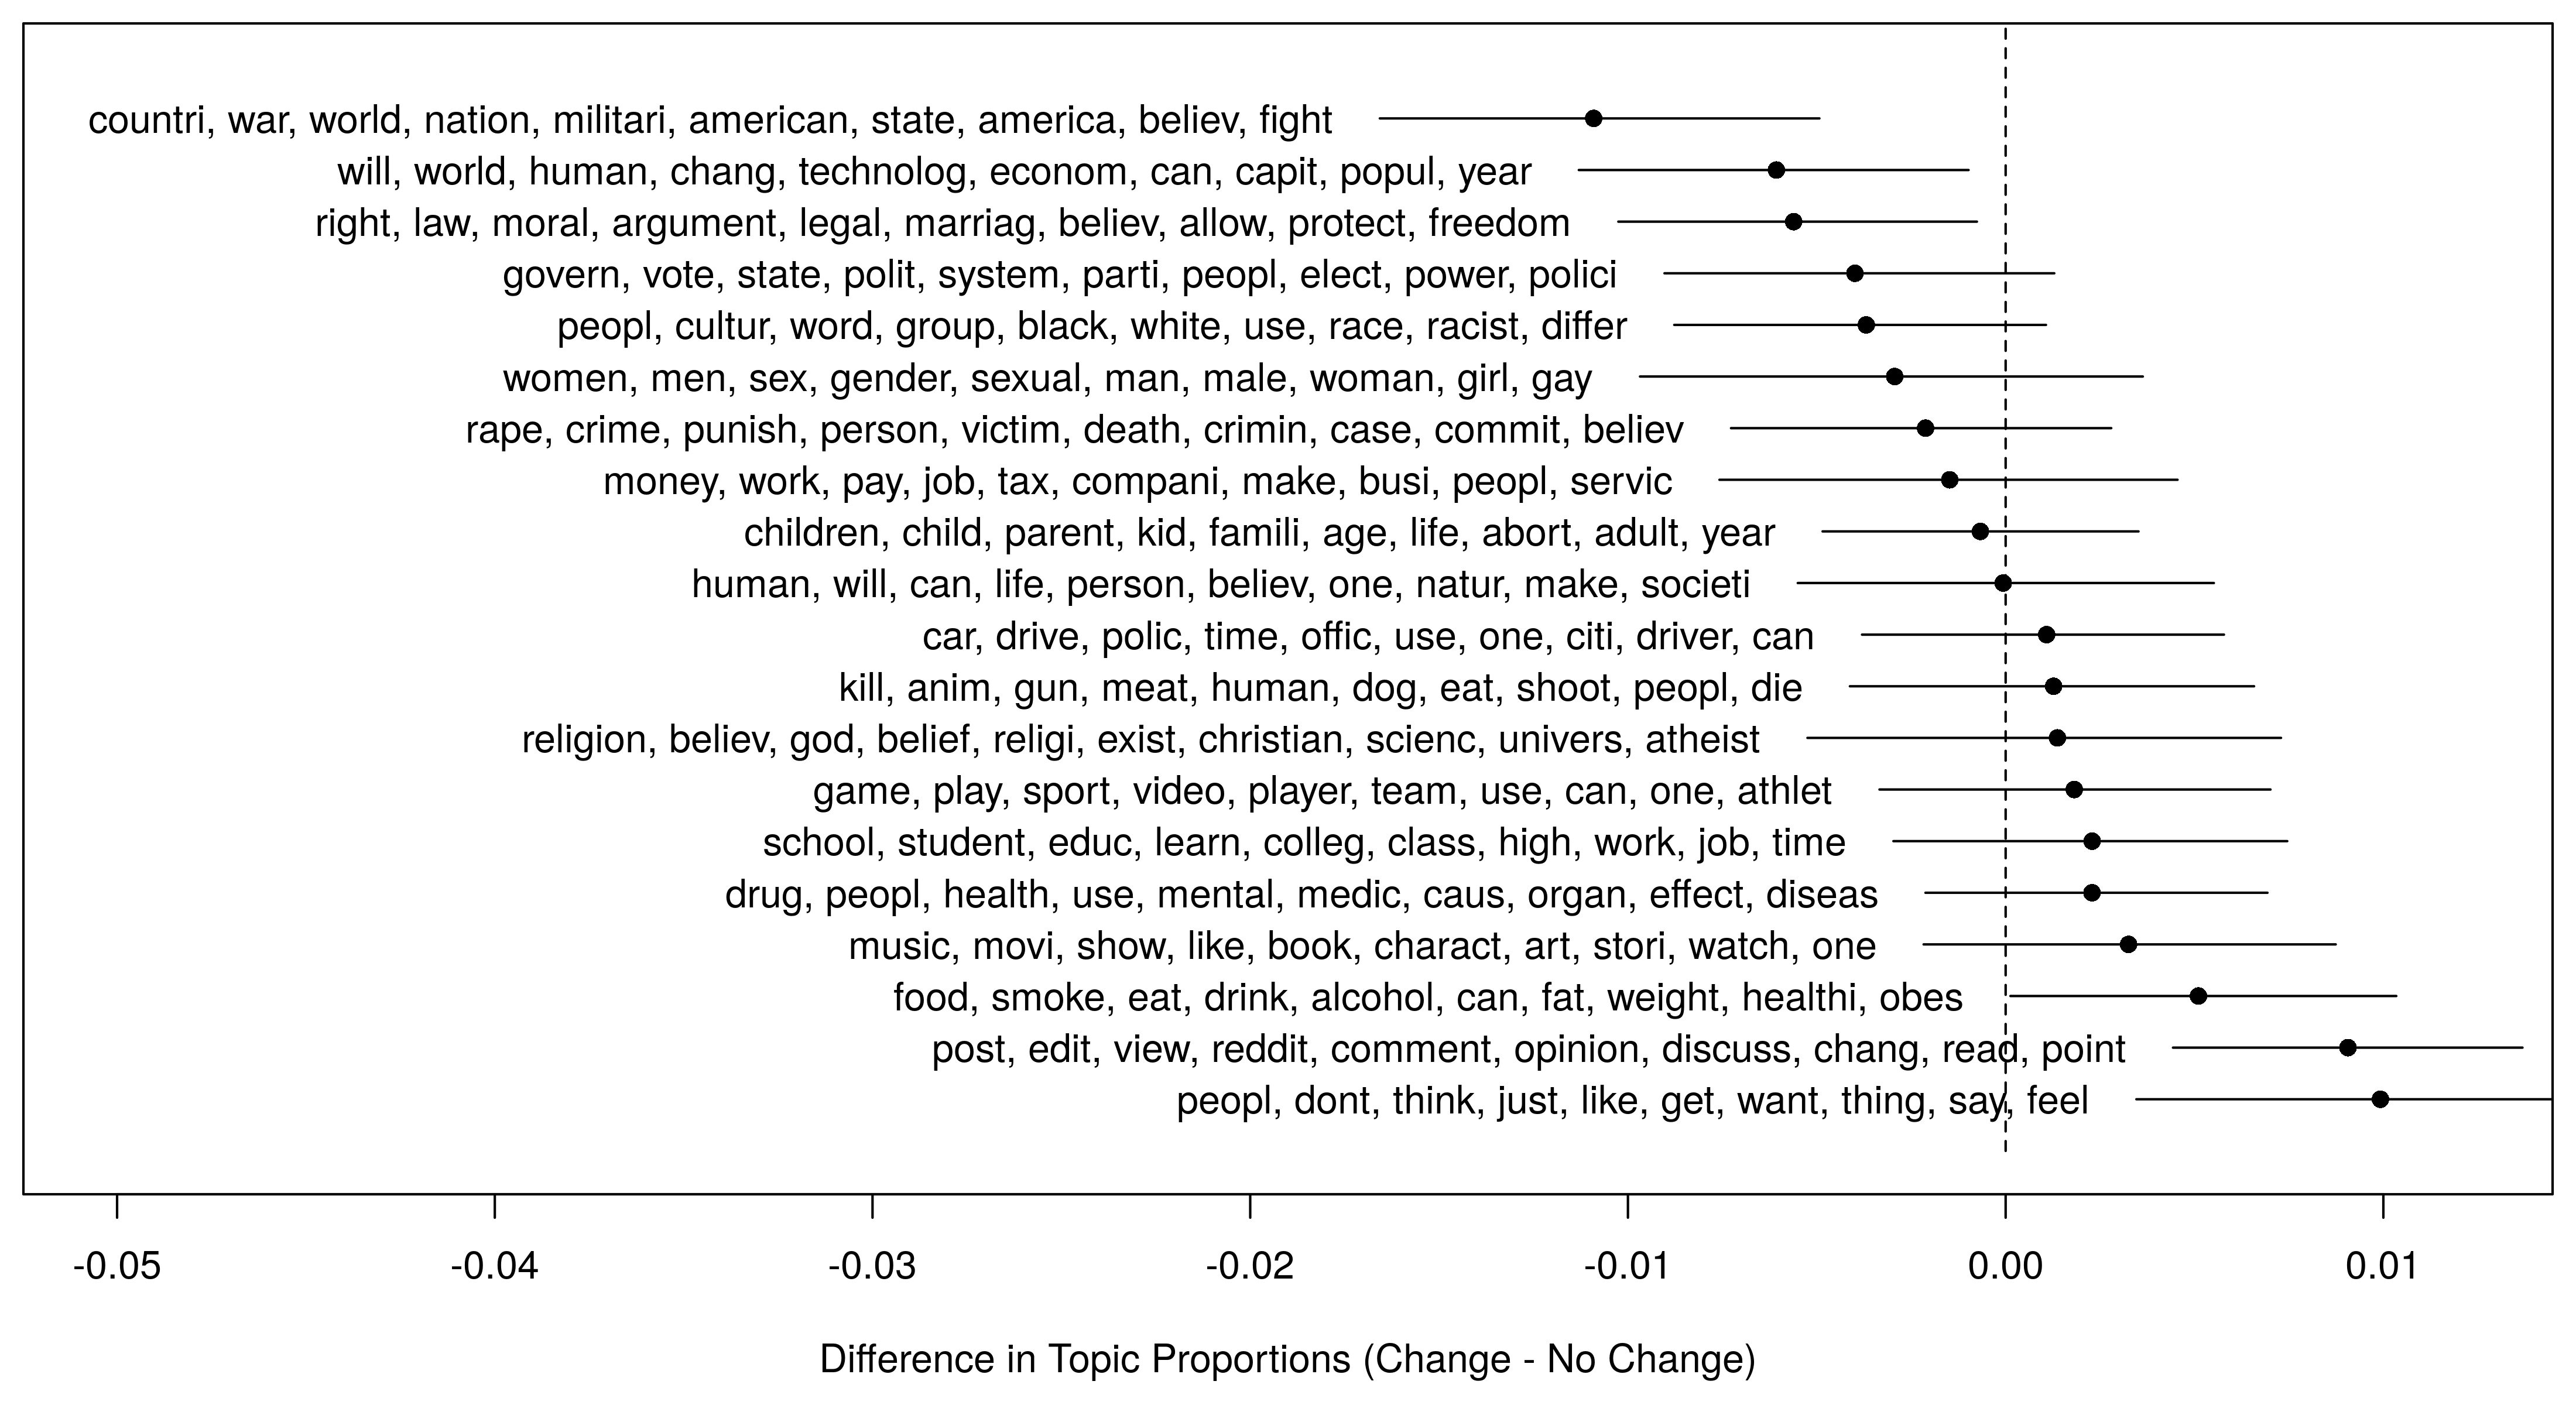
\includegraphics[width=\textwidth]{../calc/fig/stm_op_diff.png}
\end{figure}
\end{frame}

\section{Overall Moral Language in Opening Statements that Awarded a $\Delta$}
\begin{frame}{Overall Moral Language in Opening Statements that Awarded a $\Delta$}
\begin{figure}
	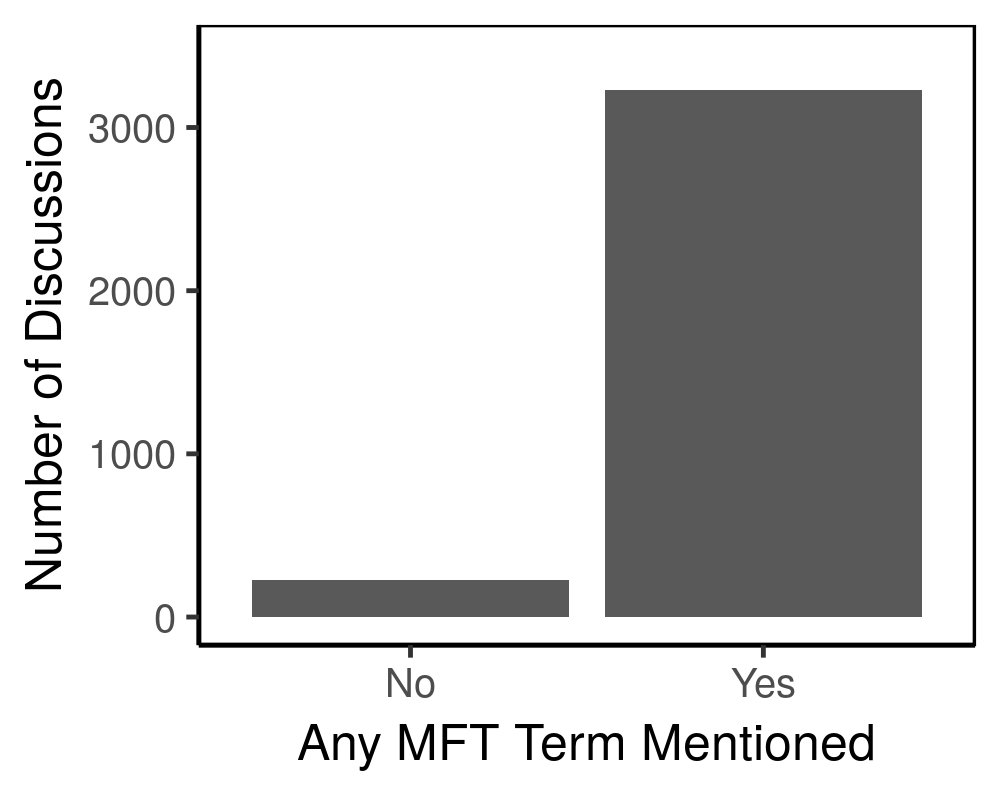
\includegraphics{../calc/fig/mft_op_all.png}
\end{figure}
\end{frame}

\section{Individual Moral Foundations in Opening Statements that Awarded a $\Delta$}
\begin{frame}{Individual Moral Foundations in Opening Statements that Awarded a $\Delta$}
\begin{figure}
	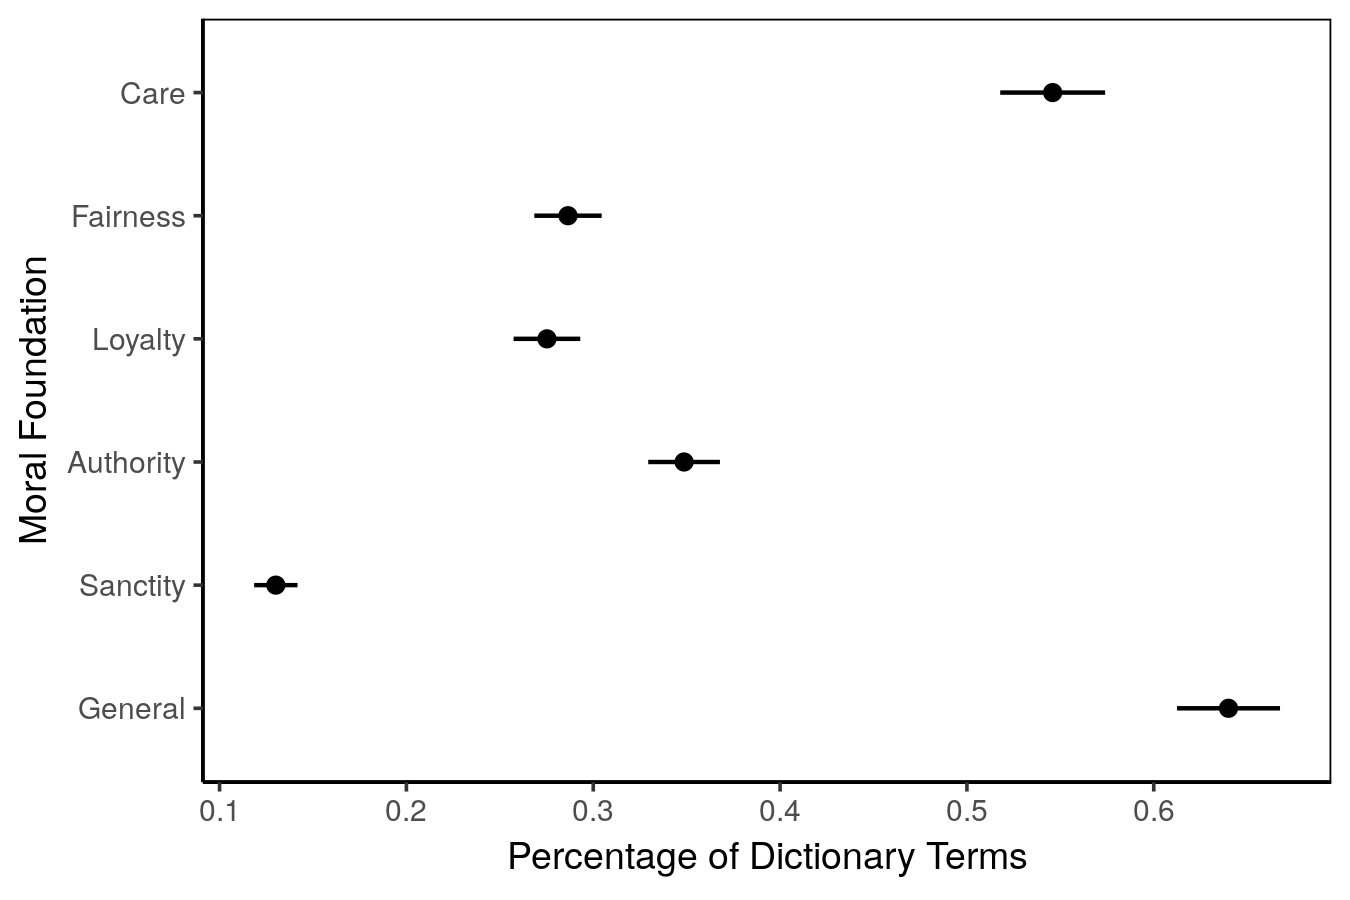
\includegraphics{../calc/fig/mft_op_individual.png}
\end{figure}
\end{frame}

\section{Argument Length and Persuasiveness}
\begin{frame}{Argument Length and Persuasiveness}
\begin{figure}
	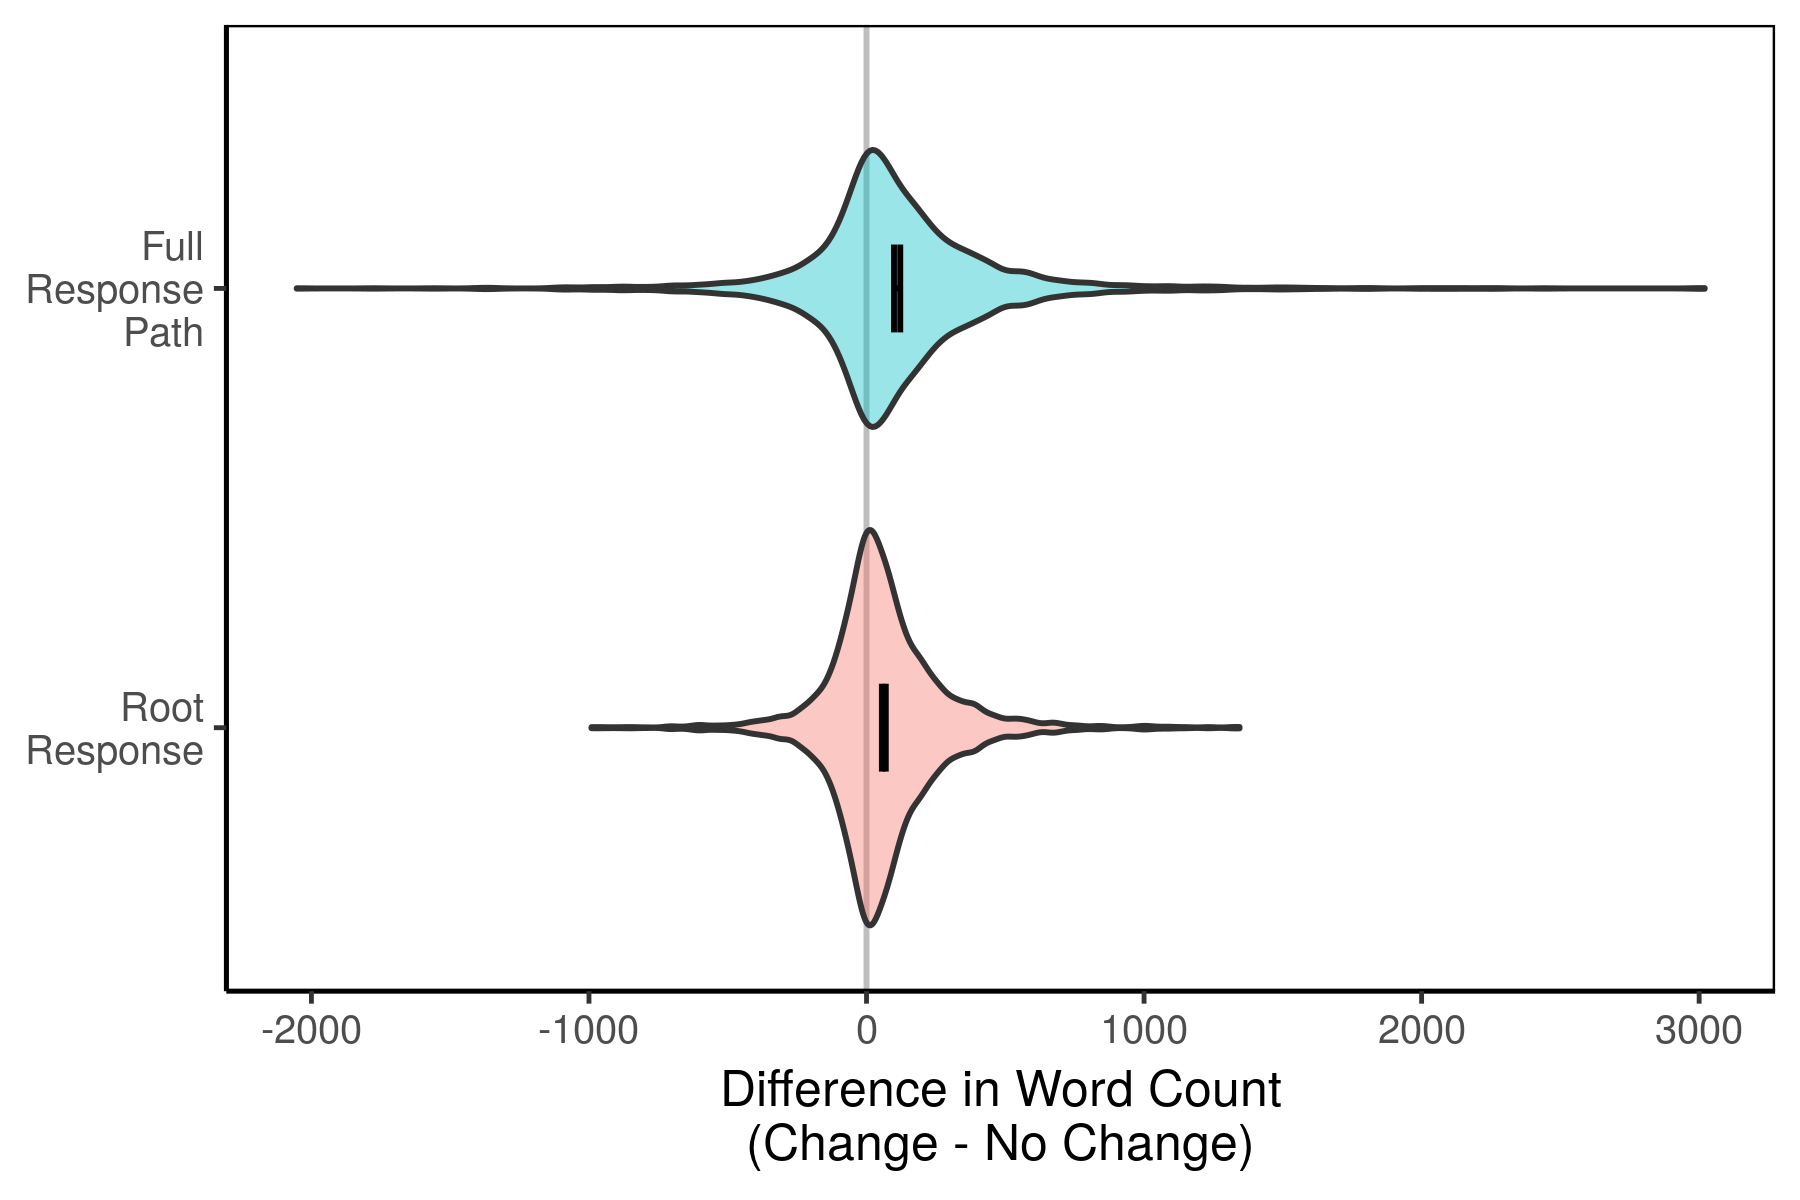
\includegraphics{../calc/fig/wordcount_violin.png}
\end{figure}
\end{frame}


\section{References}
\begin{frame} %<beamer:0> % hide references
  \frametitle{References}
  \def\newblock{\hskip .11em plus .33em minus .07em}
  %\nocite{*}
  \begin{scriptsize}
    \bibliographystyle{/data/Dropbox/Uni/Lit/apsr2006}
    \bibliography{/data/Dropbox/Uni/Lit/Literature}
  \end{scriptsize}
\end{frame}

\end{document}